% !TEX root = ../OT4ML.tex

%%%%%%%%%%%%%%%%%%%%%%%%%%%%%%%%%%%%%%%%%%%%%%%%%%%%%%%%%%%%%%%%%%%%%%%%%%%
%%%%%%%%%%%%%%%%%%%%%%%%%%%%%%%%%%%%%%%%%%%%%%%%%%%%%%%%%%%%%%%%%%%%%%%%%%%
%%%%%%%%%%%%%%%%%%%%%%%%%%%%%%%%%%%%%%%%%%%%%%%%%%%%%%%%%%%%%%%%%%%%%%%%%%%
\chapter{Kantorovich Relaxation}
\index{Kantorovich!relaxation}% strictindex
\label{sec-kantorovich}

Kantorovich's relaxation is the decisive move that turns transport into convex optimization. This chapter replaces deterministic maps by couplings, first for discrete histograms and then for general measures; it develops the resulting linear-programming structure, existence theory and characterization of optimizers by cyclical monotonicity. The metric geometry induced when the cost is a power of a ground distance is the subject of the next chapter. Historically, this viewpoint grew from Kantorovich's economic planning work~\cite{Kantorovich42} and is now the standard foundation of OT~\cite{Villani03,Villani09,rachev1998mass2}.

%%%%%%%%%%%%%%%%%%%%%%%%%%%%%%%%%%%%%%%%%%%%%%%%%%%%%%%%%%%%%%%%%%%%%%%%%%%
\section{Discrete Relaxation}
\label{sec-discrete-relaxation}

The discrete relaxation is the cleanest place to see mass splitting. It replaces permutations by a transportation polytope and reveals the linear-programming structure that algorithms exploit.
\index{transportation polytope}% strictindex

\paragraph{Mass splitting and couplings.}
\index{mass!splitting}% strictindex

Monge's discrete matching problem is problematic because it cannot be applied when $n \neq m$. A faithful formulation must keep track of masses $(\a_i,\b_j)$. The continuous Monge problem~\eqref{eq-monge-continuous}, based on push-forward maps, has the same obstruction in another form: there may be no map $T$ such that $T_\sharp\al=\be$. This happens, for instance, when a single Dirac mass should be sent to several Dirac masses.
\index{assignment problem}% strictindex
\index{Monge!problem}% strictindex
\index{push-forward}% strictindex
\index{Dirac mass}% strictindex

This lack of mass splitting also makes the Monge formulation asymmetric in $\al$ and $\be$: one can map two Dirac masses to a single one, but not the other way around. Even when a feasible map exists, the resulting optimization problem is non-convex and therefore difficult to solve numerically.

Kantorovich's key idea~\cite{Kantorovich42} is to relax the deterministic nature of transportation. Instead of requiring each source point $x_i$ to be sent to exactly one target, the mass at $x_i$ may be dispatched across several locations. This moves from deterministic transport maps to probabilistic, or fuzzy, transport plans. The relaxation is encoded, in place of a permutation $\sigma$ or a map $T$, by a coupling matrix $\P\in\RR_+^{n\times m}$, where $\P_{i,j}$ describes the amount of mass flowing from $x_i$ to $y_j$ in the formalism of discrete measures
\index{plan!transport}% strictindex
\index{transport!map}% strictindex
\[
	\al=\sum_i \a_i\de_{x_i},
	\qquad
	\be=\sum_j \b_j\de_{y_j}.
\]
\begin{defn}[Discrete couplings and mass conservation]\label{def-discrete-couplings}
\index{discrete!coupling}% strictindex
\index{mass!conservation}% strictindex
	Admissible couplings are only constrained to satisfy conservation of mass:
	\eql{\label{eq-discr-couplings}
		\CouplingsD(\a,\b)
		\eqdef
		\enscond{\P\in\RR_+^{n\times m}}{\P\ones_m=\a \qandq \transp{\P}\ones_n=\b}.
	}
	Equivalently,
	\[
		\P\ones_m=\bigl(\sum_j \P_{i,j}\bigr)_i\in\RR^n,
		\qquad
		\transp{\P}\ones_n=\bigl(\sum_i \P_{i,j}\bigr)_j\in\RR^m.
	\]
\end{defn}
\begin{rem}[Small transportation polytopes]\label{rem-small-transportation-polytopes}
\index{transportation polytope}% strictindex
\index{discrete!coupling}% strictindex
	The definition is already informative in the smallest dimensions. If $n=m=1$, mass conservation fixes the only entry, so the feasible set is a singleton. The same happens for $(n,m)=(2,1)$, and by symmetry for $(n,m)=(1,2)$: the unique coupling is forced by its only column, or by its only row.

	The first nontrivial case is $(n,m)=(2,2)$. Let $\a=(p,1-p)$ and $\b=(q,1-q)$ with $p,q\in[0,1]$. Once $s\eqdef \P_{1,1}$ is chosen, the marginal constraints force all other entries, hence every coupling has the form
	\[
		\P(s)=
		\begin{pmatrix}
			s & p-s \\
			q-s & 1-p-q+s
		\end{pmatrix}.
	\]
	The nonnegativity constraints are exactly $s\in[\max(0,p+q-1),\min(p,q)]$, so $\CouplingsD(\a,\b)$ is a segment, possibly reduced to a point at the boundary. In general, when all marginal entries are positive, the transportation polytope has affine dimension $(n-1)(m-1)$ before the nonnegativity inequalities cut out its faces.
\end{rem}
The first useful consequence of this relaxation is feasibility: there is always at least one admissible plan, obtained by making source and target independent.

\begin{defn}[Discrete product coupling]\label{def-discrete-product-coupling}
\index{product!coupling}% strictindex
	Given weights $\a\in\simplex_n$ and $\b\in\simplex_m$, the discrete product, or trivial, coupling is
	\[
		(\a\otimes\b)_{i,j}\eqdef \a_i\b_j.
	\]
	It belongs to $\CouplingsD(\a,\b)$ and corresponds to choosing the source and target labels independently.
\end{defn}
This feasible set is the bounded intersection of an affine space with the nonnegative orthant, hence a convex polytope. In one dimension, an ordered coupling can be read as a matrix: rows index source bins, columns index target bins, and the marginal constraints appear as prescribed row and column sums.
\index{marginal!constraint}% strictindex

\begin{prop}[Discrete product optimality is degenerate]\label{prop-discrete-product-coupling-degenerate}
\index{product!coupling}% strictindex
	Assume that the zero-mass rows and columns have been removed, so that $\a_i>0$ and $\b_j>0$, and let $\C$ be a finite cost matrix. The product plan $\a\otimes\b$ minimizes $\P\mapsto\dotp{\C}{\P}$ over $\CouplingsD(\a,\b)$ if and only if every coupling $\P\in\CouplingsD(\a,\b)$ minimizes it.
\index{cost!matrix}% strictindex
\end{prop}
\begin{proof}
	The reverse implication is immediate. Assume conversely that $\a\otimes\b$ is optimal and let $\Q\in\CouplingsD(\a,\b)$ be arbitrary. Since all entries of $\a\otimes\b$ are positive, there exists $t>0$ small enough that
	\(\R\eqdef (1+t)(\a\otimes\b)-t\Q\)
	has nonnegative entries. Its row and column sums are $\R\ones_m=(1+t)\a-t\a=\a$ and $\R^\top\ones_n=(1+t)\b-t\b=\b$, so $\R\in\CouplingsD(\a,\b)$. Moreover,
	\(\a\otimes\b=\frac{1}{1+t}\R+\frac{t}{1+t}\Q\).
	By optimality of $\a\otimes\b$, both $\dotp{\C}{\R}$ and $\dotp{\C}{\Q}$ are at least $\dotp{\C}{\a\otimes\b}$. Taking the scalar product of the convex-combination identity with $\C$ gives
	\[
		\dotp{\C}{\a\otimes\b}
		=
		\frac{1}{1+t}\dotp{\C}{\R}
		+\frac{t}{1+t}\dotp{\C}{\Q}.
	\]
	A convex average of two numbers not smaller than $\dotp{\C}{\a\otimes\b}$ can equal $\dotp{\C}{\a\otimes\b}$ only if both numbers are equal to it. Hence $\dotp{\C}{\Q}=\dotp{\C}{\a\otimes\b}$, and $\Q$ is optimal. Since $\Q$ was arbitrary, all couplings are optimal.
\end{proof}

Thus the product plan is mainly a feasibility witness. Except in the degenerate situation where the linear cost is constant on the whole transportation polytope, it is not expected to solve optimal transport. It is also maximally diffuse: when all masses are positive, it has $nm$ positive entries, whereas Proposition~\ref{prop-sparse-optimal-plans} shows below that sparse optimal plans with at most $n+m-1$ positive entries always exist.
\index{optimal plan}% strictindex
\index{plan!sparse}% strictindex
\index{transportation polytope}% strictindex

Figure~\ref{fig:kantorovich-coupling-polylines} contrasts deterministic, product and optimal couplings through weighted transport segments.

\begin{figure}[H]
\centering
\begin{tabular}{@{}ccc@{}}
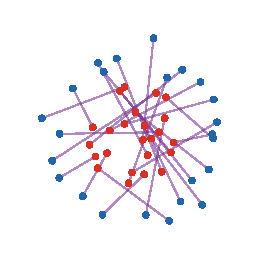
\includegraphics[width=.28\linewidth]{figures/kantorovich-coupling-polylines/graph.pdf} &
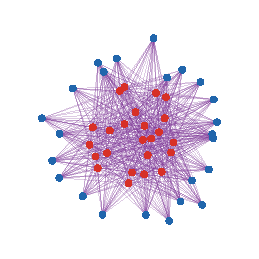
\includegraphics[width=.28\linewidth]{figures/kantorovich-coupling-polylines/product.pdf} &
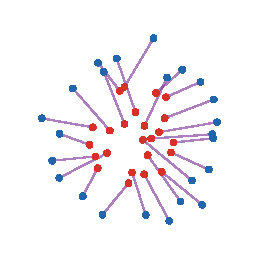
\includegraphics[width=.28\linewidth]{figures/kantorovich-coupling-polylines/optimal.pdf} \\[-.1em]
\small deterministic graph & \small product plan $\a\otimes\b$ & \small optimal plan
\end{tabular}
\caption{\emph{Discrete couplings represented as straight transport segments on the canonical point clouds used in the matching section.} The deterministic graph is a feasible Monge-type plan, the product plan spreads every source mass over all targets, and the optimal Kantorovich plan minimizes the quadratic transport cost. Line width and opacity encode the transported mass.}
\label{fig:kantorovich-coupling-polylines}
\end{figure}

Figure~\ref{fig:kantorovich-coupling-matrix-marginals} gives the complementary matrix representation and attaches the prescribed marginals directly to each plan.

\begin{figure}[H]
\centering
\begin{tabular}{@{}cccc@{}}
\small product, 20 bins & \small OT, 20 bins & \small product, 200 bins & \small OT, 200 bins \\[-.15em]
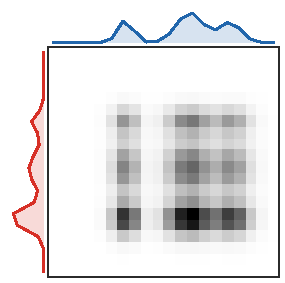
\includegraphics[width=.22\linewidth]{figures/kantorovich-coupling-matrix-marginals/product-20.pdf} &
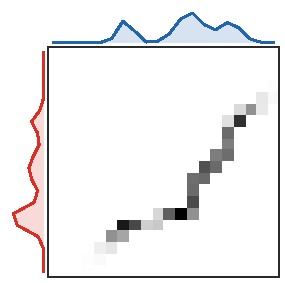
\includegraphics[width=.22\linewidth]{figures/kantorovich-coupling-matrix-marginals/optimal-20.pdf} &
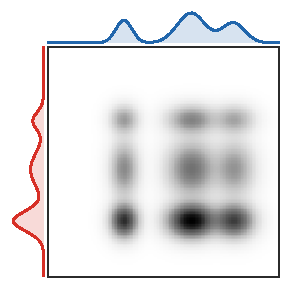
\includegraphics[width=.22\linewidth]{figures/kantorovich-coupling-matrix-marginals/product-200.pdf} &
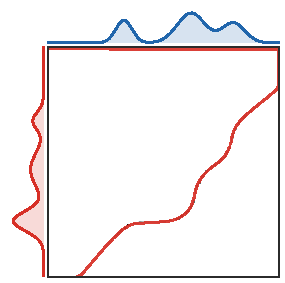
\includegraphics[width=.22\linewidth]{figures/kantorovich-coupling-matrix-marginals/optimal-200.pdf}
\end{tabular}
\caption{\emph{Coupling matrices with their prescribed marginals.} The central grayscale image displays $\P_{i,j}$; the red curve on the left is the source marginal $\a$, and the blue curve on top is the target marginal $\b$. The independent product plan is diffuse, whereas the one-dimensional optimal plan concentrates near the monotone quantile correspondence. Only the dense 200-bin optimal panel overlays the barycentric projection $i\mapsto\sum_j \P_{i,j}j/\a_i$, because that curve is meaningful visually only at sufficient resolution.}
\index{barycentric!projection}% strictindex
\index{correspondence}% strictindex
\label{fig:kantorovich-coupling-matrix-marginals}
\end{figure}

Whereas the Monge formulation is intrinsically asymmetric, Kantorovich's relaxed formulation is symmetric at the level of feasible sets: a coupling $\P$ belongs to $\CouplingsD(\a,\b)$ if and only if $\transp{\P}$ belongs to $\CouplingsD(\b,\a)$.
\index{Kantorovich!relaxation}% strictindex

\paragraph{Linear-programming structure.}
\index{linear!programming}% strictindex

Kantorovich, aiming for economic planning, made a strong simplifying assumption: the cost of transportation should be linear in the amount of transported mass.
\index{Kantorovich!problem}% strictindex
\begin{defn}[Discrete Kantorovich problem]\label{def-discrete-kantorovich-problem}
	For $\a\in\simplex_n$, $\b\in\simplex_m$, and $\C\in\RR^{n\times m}$, define
\eql{\label{eq-kanto-discr}
	\MKD_{\C}(\a,\b)
	\eqdef
	\umin{\P\in\CouplingsD(\a,\b)}
		\dotp{\C}{\P}
	=
	\umin{\P\in\CouplingsD(\a,\b)}
		\sum_{i,j}\C_{i,j}\P_{i,j}.
}
A minimizer $\P$ is an optimal coupling, or optimal transport plan.
\end{defn}
Here $\C_{i,j}$ is the cost of moving one unit of mass from $x_i$ to $y_j$.
This is a linear program, and its solutions need not be unique.

The discrete transport value has opposite curvature in its two types of data: mixing marginals gives convexity, whereas minimizing a linear objective over couplings gives concavity in the cost matrix.
\begin{prop}[Convexity in the marginals and concavity in the cost]\label{prop-discrete-kantorovich-joint-convexity}
\index{convexity!discrete OT}% strictindex
\index{concavity!discrete OT}% strictindex
	For every fixed cost matrix $\C\in\RR^{n\times m}$, the map
	\[
		(\a,\b)\longmapsto\MKD_{\C}(\a,\b)
	\]
	is jointly convex on $\simplex_n\times\simplex_m$. For every fixed $(\a,\b)\in\simplex_n\times\simplex_m$, the map
	\[
		\C\longmapsto\MKD_{\C}(\a,\b)
	\]
	is concave on $\RR^{n\times m}$.
\end{prop}

\begin{proof}
	For $r\in\{0,1\}$, let $\P_r$ be optimal between $\a_r$ and $\b_r$. For $t\in[0,1]$, the matrix $\P_t=(1-t)\P_0+t\P_1$ belongs to $\CouplingsD((1-t)\a_0+t\a_1,(1-t)\b_0+t\b_1)$. Therefore
	\[
		\MKD_{\C}\big((1-t)\a_0+t\a_1,(1-t)\b_0+t\b_1\big)
		\leq
		\dotp{\C}{\P_t}
		=
		(1-t)\MKD_{\C}(\a_0,\b_0)+t\MKD_{\C}(\a_1,\b_1).
	\]
	For fixed marginals, every $\P\in\CouplingsD(\a,\b)$ satisfies
	\[
		\dotp{(1-t)\C_0+t\C_1}{\P}
		\geq
		(1-t)\MKD_{\C_0}(\a,\b)
		+t\MKD_{\C_1}(\a,\b).
	\]
	Minimizing the left-hand side over $\P$ proves concavity in $\C$.
\end{proof}

Figure~\ref{fig:kantorovich-permutation-versus-splitting} contrasts the permutation plans inherited from equal-weight assignments with the genuinely splitting couplings permitted by nonuniform marginals.

\begin{figure}[H]
\centering
\begin{tabular}{@{}cccc@{}}
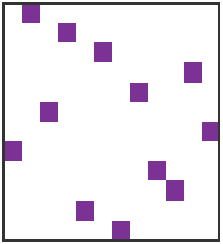
\includegraphics[width=.18\linewidth]{figures/kantorovich-permutation-versus-splitting/permutation-matrix.pdf} &
\index{matrix!permutation}% strictindex
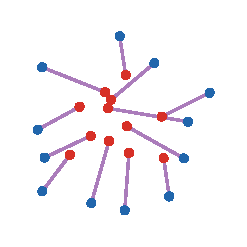
\includegraphics[width=.23\linewidth]{figures/kantorovich-permutation-versus-splitting/permutation-transport.pdf} &
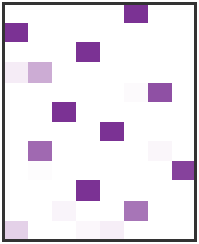
\includegraphics[width=.16\linewidth]{figures/kantorovich-permutation-versus-splitting/splitting-matrix.pdf} &
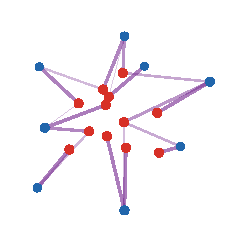
\includegraphics[width=.23\linewidth]{figures/kantorovich-permutation-versus-splitting/splitting-transport.pdf} \\[-.1em]
\small permutation matrix $\P_\sigma$ &
\small assignment segments &
\small splitting matrix $\P$ &
\small splitting segments
\end{tabular}
\caption{\emph{From permutation matrices to splitting couplings.} When the two empirical measures have the same number of atoms and uniform weights, an optimal plan can be a permutation matrix. Once target masses are nonuniform, the admissible set $\CouplingsD(\a,\b)$ also contains plans in which one source sends mass to several targets and several sources merge into the same target.}
\index{matrix!permutation}% strictindex
\index{empirical!measure}% strictindex
\label{fig:kantorovich-permutation-versus-splitting}
\end{figure}

Sparsity here is not peculiar to transport. For nonnegative variables, the relevant quantity is the rank of the constraint operator---not the raw number of listed constraints, which may contain redundancies. The following standard linear-programming principle makes this precise; see, for instance,~\cite{bertsimas1997introduction}.
\index{sparsity}% strictindex
\index{rank}% strictindex

\begin{prop}[Rank-controlled sparse minimizers]\label{prop-lp-rank-sparsity}
\index{linear!programming}% strictindex
\index{linear!operator}% strictindex
\index{minimizer!sparse}% strictindex
	Let $\mathcal A:\RR^{n\times m}\to\RR^q$ be linear, let $\mathbf d\in\RR^q$ and $\C\in\RR^{n\times m}$, and consider
	\begin{equation}\label{eq-lp-rank-sparsity}
		\inf_{\P\geq 0,\;\mathcal A(\P)\leq\mathbf d}
		\dotp{\C}{\P},
	\end{equation}
	where the inequality is componentwise. If the feasible set is nonempty and the objective is bounded below on it, then~\eqref{eq-lp-rank-sparsity} admits a minimizer $\P^\star$ satisfying
	\begin{equation}\label{eq-lp-rank-support-bound}
		\#\enscond{(i,j)}{\P^\star_{i,j}>0}
		\leq \operatorname{rank}(\mathcal A).
	\end{equation}
	Here $\operatorname{rank}(\mathcal A)=\dim(\operatorname{Im}\mathcal A)$. The same conclusion holds when $\mathcal A(\P)\leq\mathbf d$ is replaced by $\mathcal A(\P)=\mathbf d$.
\end{prop}

\begin{proof}
	The feasible region is a nonempty polyhedron, and the objective is bounded below on it. The attainment theorem for linear programs therefore provides a minimizer. Among all minimizers, choose $\P^\star$ with the smallest number of positive entries, and denote its support by $S$.

	Suppose that $\#S>\operatorname{rank}(\mathcal A)$. The restriction of $\mathcal A$ to the $\#S$-dimensional space of matrices supported on $S$ then has a nontrivial kernel. Hence there is a nonzero matrix $H$, supported on $S$, such that $\mathcal A(H)=0$. Since $\P^\star$ is strictly positive on $S$, both $\P^\star+tH$ and $\P^\star-tH$ remain nonnegative for all sufficiently small $t>0$. Moreover, $\mathcal A(\P^\star\pm tH)=\mathcal A(\P^\star)$, so both perturbations satisfy exactly the same linear inequalities, or equalities, as $\P^\star$. Optimality forces $\dotp{\C}{H}=0$; otherwise one of the two signs would strictly decrease the objective.

	Choose $\sigma\in\{-1,1\}$ such that $\sigma H$ has a negative entry, and set $t_\star\eqdef\min_{(i,j):\,\sigma H_{i,j}<0}\P^\star_{i,j}/(-\sigma H_{i,j})>0$.
	Then $\P^\star+t_\star\sigma H$ is nonnegative, feasible, and has the same cost as $\P^\star$. At least one of its positive entries has become zero, while no new entry has appeared outside $S$. This contradicts the minimality of $S$ and proves~\eqref{eq-lp-rank-support-bound}.
\end{proof}

\begin{prop}[Sparse optimal plans]\label{prop-sparse-optimal-plans}
\index{optimal plan}% strictindex
\index{plan!sparse}% strictindex
	Assume $\a_i>0$, $\b_j>0$ and $\sum_i \a_i=\sum_j \b_j=1$. The linear program~\eqref{eq-kanto-discr} admits an optimal coupling with at most $n+m-1$ nonzero entries.
\index{optimal coupling}% strictindex
\end{prop}
\begin{proof}
	The transportation polytope is nonempty and compact, so the minimum is finite. Apply the equality case of Proposition~\ref{prop-lp-rank-sparsity} to the marginal operator $\mathcal A_{\mathrm{marg}}(\P)\eqdef(\P\ones_m,\transp{\P}\ones_n)\in\RR^{n+m}$.
	Its rank is $n+m-1$. Indeed, every matrix satisfies
	$\sum_i(\P\ones_m)_i=\sum_j(\transp{\P}\ones_n)_j$, so there is one linear dependence among the $n+m$ marginal coordinates. It is the only one: if $u\in\RR^n$ and $v\in\RR^m$ satisfy
	\[
		\dotp{u}{\P\ones_m}
		+
		\dotp{v}{\transp{\P}\ones_n}=0
		\qquad\text{for every }\P,
	\]
	then testing this identity on each elementary matrix gives $u_i+v_j=0$ for every $(i,j)$. Thus all $u_i$ equal one scalar and all $v_j$ equal its opposite, so the annihilator of $\operatorname{Im}(\mathcal A_{\mathrm{marg}})$ is one-dimensional. It follows that $\operatorname{rank}(\mathcal A_{\mathrm{marg}})=n+m-1$, and Proposition~\ref{prop-lp-rank-sparsity} supplies the claimed optimal coupling.
\end{proof}

For transportation polytopes, this rank argument also has a graph interpretation. A cycle in the bipartite support produces an alternating nonzero perturbation with zero row and column sums, exactly the kernel direction used in the general proof. Consequently, the positive support of an extreme coupling is a forest.
\index{graph!support}% strictindex
\index{graph!bipartite}% strictindex

\begin{prop}[North-west corner feasible plan]\label{prop-northwest-corner}
\index{north-west corner!plan}% strictindex
	Let $\a\in\RR_+^n$ and $\b\in\RR_+^m$ have the same positive total mass. The following greedy sweep constructs a coupling $\P\in\CouplingsD(\a,\b)$ with at most $n+m-1$ positive entries and an acyclic positive support. Starting from $(i,j)=(1,1)$ with residual masses $r_i=\a_i$ and $s_j=\b_j$, skip zero residuals, set $\P_{i,j}=\min(r_i,s_j)$,
\index{greedy sweep}% strictindex
	subtract this value from both residuals, and advance every index whose residual has become zero. Repeat until all residual masses are exhausted.
\end{prop}
\begin{proof}
	All assignments are nonnegative. At each step, the mass placed in entry $(i,j)$ is subtracted from exactly one current row residual and one current column residual, so no row or column can receive more mass than prescribed. Conversely, an index is advanced only when its residual has been fully filled. When the algorithm stops, the total assigned mass is $\sum_i \a_i=\sum_j \b_j$, hence all row and column sums are exactly $\a$ and $\b$.

	Each positive assignment exhausts at least one current row or one current column. Before the final assignment, at most $n-1$ row advances and $m-1$ column advances can occur without terminating the construction. Hence the number of positive entries is at most $(n-1)+(m-1)+1=n+m-1$. For acyclicity, view the positive support as a bipartite graph. Once a row or column index is advanced, it never appears again, so each new positive edge either starts a new component or attaches at least one new vertex to the component currently being swept. No edge is ever added between two old vertices of the same component, so no cycle can be created.
\index{graph!bipartite}% strictindex
\end{proof}

\begin{alg}[North-west corner coupling]\label{alg:north-west-corner}
\textbf{Input:} Source weights $\a\in\simplex_n$ and target weights $\b\in\simplex_m$.

\textbf{Output:} Sparse feasible coupling $\P\in\CouplingsD(\a,\b)$.

\textbf{Initialize:} Set $\P=0$, $r=\a$, $s=\b$, and $(i,j)=(1,1)$.

\textbf{While} $i\leq n$ and $j\leq m$ \textbf{do}:
\begin{algblock}
\(\eta=\min(r_i,s_j), \qquad \P_{i,j}\leftarrow \eta.\)

\textbf{Update residuals:}
\(r_i\leftarrow r_i-\eta, \qquad s_j\leftarrow s_j-\eta.\)

\textbf{If} $r_i=0$ \textbf{then}:
\begin{algblock}

\textbf{Set} $i\leftarrow i+1$.

\end{algblock}
\textbf{If} $s_j=0$ \textbf{then}:
\begin{algblock}

\textbf{Set} $j\leftarrow j+1$.

\end{algblock}
\end{algblock}
\algreturnskip
\textbf{Return} $\P$.
\end{alg}

The north-west corner rule, summarized in Algorithm~\ref{alg:north-west-corner}, does not use the cost matrix and is therefore not meant to solve~\eqref{eq-kanto-discr}. Its role is algorithmic: an acyclic support corresponds to linearly independent marginal constraints. When the support has fewer than $n+m-1$ positive entries, transportation simplex implementations complete it with zero-mass basic variables to obtain a degenerate basic feasible solution. This gives a cheap initialization for the pivoting methods discussed in Section~\ref{sec-kantorovich-lp-algorithms}.
\index{cost!matrix}% strictindex
\index{north-west corner!rule}% strictindex
\index{basic feasible solution}% strictindex
\index{transportation simplex}% strictindex
\index{marginal!constraint}% strictindex

\paragraph{One-dimensional cases.}
\index{one-dimensional!transport}% strictindex

In one dimension, the transportation polytope has a canonical monotone optimizer. This is the weighted version of the sorting rule from Section~\ref{sec-monge-pbm}.
\index{transportation polytope}% strictindex

\begin{prop}[One-dimensional weighted sweep]\label{prop-1d-weighted-sweep}
\index{weighted!sweep}% strictindex
	Let $x_1\leq\cdots\leq x_n$ and $y_1\leq\cdots\leq y_m$ be points on the line, and let $c(x,y)=h(x-y)$ with $h$ convex. The north-west corner plan between the sorted weighted atoms is optimal for~\eqref{eq-kanto-discr}. Consequently, for unsorted one-dimensional inputs, an optimal plan is obtained in $O(n\log n+m\log m)$ time by sorting and then sweeping the masses once from left to right.
\index{optimal plan}% strictindex
\index{north-west corner!plan}% strictindex
\end{prop}
\begin{proof}
		The north-west plan is monotone: if $i<i'$ and $j>j'$, it cannot put positive mass on both $(i,j)$ and $(i',j')$, because the sweep exhausts rows and columns in increasing order. To prove optimality, start from an arbitrary feasible plan $\P$. If
		$\P_{1,1}<\min(\a_1,\b_1)$, then row $1$ sends positive mass to some column $j>1$, while column $1$ receives positive mass from some row $i>1$. Moving
		\(\eta=\min(\P_{1,j},\P_{i,1})\)
		from $(1,j)$ and $(i,1)$ to $(1,1)$ and $(i,j)$ preserves both marginals. Convexity of $h$ gives the Monge inequality
		\[
			h(x_1-y_j)+h(x_i-y_1)
			\geq
			h(x_1-y_1)+h(x_i-y_j),
		\]
		so this exchange does not increase the cost. Each exchange either removes the chosen entry in row $1$ or removes the chosen entry in column $1$. Repeating finitely many times forces
		$\P_{1,1}=\min(\a_1,\b_1)$, exactly the first north-west assignment. It exhausts row $1$, column $1$, or both. Removing every exhausted index reduces the problem to a smaller ordered transportation problem. Induction on $n+m$ produces the complete north-west plan without increasing cost. Sorting costs $O(n\log n+m\log m)$ and the sweep uses at most $n+m-1$ positive assignments.
\end{proof}


\paragraph{Permutation matrices as couplings.}
\index{matrix!permutation}% strictindex

We now restrict attention to the special case $n=m$ and uniform weights $\a=\b=\ones_n/n$. In this case a matching can be encoded as a matrix with exactly one active entry per row and per column.

\begin{defn}[Permutation matrices]\label{def-permutation-matrices}
\index{permutation matrix}% strictindex
	For a permutation $\sigma\in\Perm(n)$, its permutation matrix $\P_\sigma$ is
	\[
		(\P_\sigma)_{i,j}=\choice{1 \qifq j=\sigma(i),\\ 0 \quad\text{otherwise}.}
	\]
	The set of all permutation matrices is
	\[
		\mathcal P_n^{\mathrm{perm}}
		\eqdef
		\enscond{\P_\sigma}{\sigma\in\Perm(n)} .
	\]
\end{defn}
The corresponding probability coupling is $\P_\sigma/n$. If the matching cost matrix is $\C$, then
\index{cost!matrix}% strictindex
\[
	\dotp{\C}{\P_\sigma/n}=\frac1n\sum_{i=1}^n \C_{i,\sigma(i)}.
\]
Thus the assignment problem is the minimization of a linear function over the discrete, non-convex set of permutation matrices.
\index{matrix!permutation}% strictindex
\index{assignment problem}% strictindex

The convex relaxation replaces this finite set by all bistochastic matrices.

\begin{defn}[Birkhoff polytope]\label{def-birkhoff-polytope}
\index{bistochastic matrix}% strictindex
\index{Birkhoff!polytope}% strictindex
	The Birkhoff polytope is the convex set of bistochastic matrices
	\[
		\mathcal B_n
		\eqdef
		\enscond{\P\in\RR_+^{n\times n}}{\P\ones_n=\ones_n \qandq \transp{\P}\ones_n=\ones_n}.
	\]
\end{defn}
Then $\CouplingsD(\ones_n/n,\ones_n/n)=\mathcal B_n/n$, and permutation couplings are included in this convex relaxation. More precisely,
\[
	\mathcal P_n^{\mathrm{perm}}
	=
	\mathcal B_n\cap\{0,1\}^{n\times n}
	\subset
	\mathcal B_n,
\]
so before using the structure of $\mathcal B_n$ one first obtains only the relaxed inequality
\[
	\min_{\P\in\mathcal B_n}\dotp{\C}{\P}
	\leq
	\min_{\P\in\mathcal P_n^{\mathrm{perm}}}\dotp{\C}{\P}.
\]
The next elementary facts lead to the Birkhoff--von Neumann theorem~\cite{birkhoff,vonNeumann1953assignment}, which explains why this relaxation is tight for uniform matching.
\index{Birkhoff!von Neumann theorem}% strictindex
\index{matching!uniform}% strictindex

\begin{defn}[Extreme points]\label{def-extreme-points}
\index{extreme point}% strictindex
		For a convex set $\mathcal C$ in a finite-dimensional vector space,
	\[
		\operatorname{Extr}(\mathcal C)
		\eqdef
		\enscond{x\in\mathcal C}{x=(y+z)/2,\ y,z\in\mathcal C \Rightarrow y=z=x}.
	\]
\end{defn}

\begin{prop}[Existence of extreme points]\label{prop-extreme-point-existence}
\index{extreme point}% strictindex
	If $\mathcal C$ is a non-empty compact convex subset of a finite-dimensional vector space, then $\operatorname{Extr}(\mathcal C)$ is non-empty.
\end{prop}
\begin{proof}
	Among all non-empty faces of $\mathcal C$, choose one of minimal affine dimension. If this face contained two distinct points, maximizing a linear functional that is not constant on the face would produce a non-empty proper exposed subface, contradicting minimality. Hence the minimal face is a singleton, and its point is extreme.
\end{proof}

\begin{example}[An unbounded convex set without extreme points]
		Compactness cannot be dropped from Proposition~\ref{prop-extreme-point-existence}. For instance, the affine line $\mathcal C=\RR\times\{0\}\subset\RR^2$ is closed, convex and unbounded, but it has no extreme point: every $(x,0)$ is the midpoint of the distinct points $(x-1,0)$ and $(x+1,0)$.
\index{extreme point}% strictindex
\end{example}

\begin{prop}[Linear programs have extreme minimizers]\label{prop-linear-program-extreme-minimizer}
\index{extreme minimizer}% strictindex
\index{linear!programming}% strictindex
		Let $\mathcal C$ be a non-empty compact convex set. For every linear form $\ell$,
\index{linear!form}% strictindex
	\[
		\operatorname{Extr}(\mathcal C)\cap\operatorname*{argmin}_{x\in\mathcal C}\ell(x)
		\neq\emptyset.
	\]
\end{prop}
\begin{proof}
	The set $S=\operatorname*{argmin}_{x\in\mathcal C}\ell(x)$ is non-empty, compact and convex. By Proposition~\ref{prop-extreme-point-existence}, it has an extreme point $x$. If $x=(y+z)/2$ with $y,z\in\mathcal C$, then by linearity and optimality of $x$, both $y$ and $z$ also minimize $\ell$ on $\mathcal C$, hence $y,z\in S$. Since $x$ is extreme in $S$, $y=z=x$. Thus $x$ is extreme in $\mathcal C$.
\index{extreme point}% strictindex
\end{proof}

\begin{thm}[Birkhoff--von Neumann]\label{thm-birkhoff-von-neumann}
\index{Birkhoff!von Neumann theorem}% strictindex
	The extreme points of $\mathcal B_n$ are exactly the permutation matrices.
\end{thm}

Figure~\ref{fig:birkhoff-von-neumann-cycle} shows the non-extreme mechanism used in the proof below. The displayed matrix is bistochastic but not a permutation matrix: the three unit entries already behave like isolated matching edges, while the scattered fractional support contains a longer alternating cycle.

\begin{figure}[ht]
\centering
\setlength{\tabcolsep}{4pt}
\begin{tabular}{@{}cc@{}}
\begin{minipage}[c]{.31\linewidth}
\centering
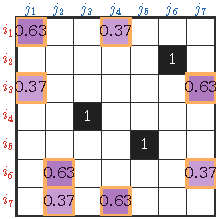
\includegraphics[width=.94\linewidth]{figures/birkhoff-von-neumann-cycle/matrix.pdf}\\[-.45em]
bistochastic matrix
\end{minipage}
&
\begin{minipage}[c]{.32\linewidth}
\centering
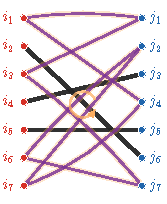
\includegraphics[width=.76\linewidth]{figures/birkhoff-von-neumann-cycle/support-graph.pdf}\\[-.45em]
support graph
\end{minipage}
\end{tabular}
\caption{\emph{Cycle certificate in the Birkhoff--von Neumann proof.} The left panel is a $7\times7$ bistochastic matrix which is not a permutation matrix. It has only three isolated entries equal to one, while the non-binary entries are scattered across four rows and columns. The right panel shows the bipartite positive-support graph, with the column nodes sorted as $j_1,\ldots,j_7$ from top to bottom to match the matrix order: red nodes are rows, blue nodes are columns, thin purple edges correspond to $0<\P_{i,j}<1$, and bold black edges correspond to isolated entries $\P_{i,j}=1$. The orange halo marks the longer alternating fractional cycle along which one can add and subtract mass while preserving all row and column sums.}
\label{fig:birkhoff-von-neumann-cycle}
\end{figure}

\begin{proof}
	We first prove that permutation matrices are extreme. Let $\P_\sigma\in\mathcal P_n^{\mathrm{perm}}$ and assume that $\P_\sigma=(\Q+\R)/2$ with $\Q,\R\in\mathcal B_n$.
	Every bistochastic matrix has entries in $[0,1]$. Since the only extreme points of $[0,1]$ are $0$ and $1$, each entry of $\P_\sigma$ fixes the corresponding entries of $\Q$ and $\R$: if $(\P_\sigma)_{i,j}=0$, then $\Q_{i,j}=\R_{i,j}=0$, while if $(\P_\sigma)_{i,j}=1$, then $\Q_{i,j}=\R_{i,j}=1$. Hence $\Q=\R=\P_\sigma$, so $\P_\sigma$ is extreme.
	\index{matrix!permutation}% strictindex

	We now prove the converse by contrapositive. Pick $\P\in\mathcal B_n\setminus\mathcal P_n^{\mathrm{perm}}$. Since an integral bistochastic matrix is necessarily a permutation matrix, $\P$ has at least one fractional entry. We shall split
	\(\P=\frac{\Q+\R}{2}\)
	with $\Q,\R\in\mathcal B_n$ and $\Q\neq \R$, proving that $\P$ is not extreme.

	Associate with $\P$ the bipartite graph whose left vertices are the rows, whose right vertices are the columns, and whose edges are the fractional entries
	\(0<\P_{i,j}<1\).
	An entry equal to $1$ uses the whole mass of its row and column, so it is isolated in the positive support and does not appear in this fractional graph. If a left vertex $i$ is incident to a fractional edge $(i,j_1)$, then it must be incident to at least one other fractional edge. Indeed, the row sum is one; after the contribution $\P_{i,j_1}\in(0,1)$, a positive amount $1-\P_{i,j_1}$ remains in the same row, and it cannot be carried by an entry equal to $1$. The same argument applies to right vertices, using the column sums. Thus every non-isolated vertex of the fractional graph has degree at least two.

	Starting from any fractional edge, one may therefore walk through adjacent fractional edges without immediately backtracking and without getting stuck. Since the graph is finite, some vertex is eventually visited twice; the portion of the walk between the two visits contains a cycle. Choose a shortest such cycle and write it in alternating form $(i_1,j_1,i_2,j_2,\ldots,i_p,j_p)$, with $i_{p+1}=i_1$, where both $(i_s,j_s)$ and $(i_{s+1},j_s)$ are fractional for every $s$. The minimality of the cycle implies that the vertices $i_s$ are all distinct and that the vertices $j_s$ are all distinct. In particular,
	\[
		0<\P_{i_s,j_s}<1
		\qandq
		0<\P_{i_{s+1},j_s}<1 .
	\]
	Define
	\[
		\epsilon
		\eqdef
		\min_{1\leq s\leq p}
		\bigl\{
		\P_{i_s,j_s},\,
		\P_{i_{s+1},j_s},\,
		1-\P_{i_s,j_s},\,
		1-\P_{i_{s+1},j_s}
		\bigr\}.
	\]
	All these numbers are positive, so $\epsilon>0$. Split the cycle edges into the two alternating families
	\[
		A\eqdef \{(i_s,j_s)\}_{s=1}^p,
		\qquad
		B\eqdef \{(i_{s+1},j_s)\}_{s=1}^p .
	\]
	We now perform the standard alternating-cycle perturbation:
	\[
		\Q_{i,j}\eqdef
		\begin{cases}
			\P_{i,j}, & (i,j)\notin A\cup B,\\
			\P_{i,j}+\epsilon/2, & (i,j)\in A,\\
			\P_{i,j}-\epsilon/2, & (i,j)\in B,
		\end{cases}
		\qquad
		\R_{i,j}\eqdef
		\begin{cases}
			\P_{i,j}, & (i,j)\notin A\cup B,\\
			\P_{i,j}-\epsilon/2, & (i,j)\in A,\\
			\P_{i,j}+\epsilon/2, & (i,j)\in B .
		\end{cases}
	\]
	By the definition of $\epsilon$, all modified entries stay in $[0,1]$, so $\Q$ and $\R$ are nonnegative. Each row vertex $i_s$ of the cycle is incident to exactly one edge of $A$ and one edge of $B$; the $+\epsilon/2$ and $-\epsilon/2$ perturbations therefore cancel in that row. The same cancellation holds in each column vertex $j_s$, and all other rows and columns are unchanged. Consequently, $\Q\ones_n=\R\ones_n=\ones_n$ and $\transp{\Q}\ones_n=\transp{\R}\ones_n=\ones_n$, so $\Q,\R\in\mathcal B_n$. Finally, $\Q\neq \R$ because $\epsilon>0$ and the cycle is non-empty, while by construction $\P=(\Q+\R)/2$. Thus $\P$ is not extreme. Consequently every extreme point of $\mathcal B_n$ is integral, and every integral bistochastic matrix is a permutation matrix.
	\index{bistochastic matrix}% strictindex
	\index{graph!bipartite}% strictindex
\index{extreme point}% strictindex
\end{proof}

\begin{cor}[Kantorovich for matching]\label{cor-kantorovich-matching}
\index{Kantorovich!relaxation}% strictindex
	If $m=n$ and $\a=\b=\ones_n/n$, then the discrete Kantorovich problem~\eqref{eq-kanto-discr} admits an optimal solution of the form $\P_\sigma/n$. The associated permutation $\sigma$ solves the assignment problem of Section~\ref{sec-monge-pbm}.
\index{Kantorovich!problem}% strictindex
\index{assignment problem}% strictindex
\end{cor}
\begin{proof}
	The feasible set is $\mathcal B_n/n$. By Proposition~\ref{prop-linear-program-extreme-minimizer}, the linear objective has an optimal extreme point. Since scaling preserves extreme points and Theorem~\ref{thm-birkhoff-von-neumann} identifies the extreme points of $\mathcal B_n$, this optimizer is $\P_\sigma/n$ for some permutation $\sigma$. Its cost is exactly $n^{-1}\sum_i \C_{i,\sigma(i)}$, so $\sigma$ is an optimal assignment.
\index{linear!objective}% strictindex
\index{Birkhoff!von Neumann theorem}% strictindex
\index{extreme point}% strictindex
\end{proof}

Equivalently, for uniform empirical measures, one can always choose a permutation matrix among the minimizers of the relaxed Kantorovich problem: the relaxation is tight for assignment problems.
\index{Kantorovich!problem}% strictindex
\index{empirical!measure}% strictindex
\index{assignment problem}% strictindex
\index{matrix!permutation}% strictindex

\begin{rem}[General discrete case]
	For general input measures, one does not have equivalence between Monge and Kantorovich problems, since the Monge constraint can be empty. In finite dimension, however, the support of an optimal coupling still enjoys strong sparsity: one can choose an optimal basic feasible plan whose bipartite support is cycle-free, hence with at most $n+m-1$ nonzero entries. Figure~\ref{fig:kantorovich-permutation-versus-splitting} illustrates the difference between the tight uniform matching case and the genuinely splitting nonuniform case.
\index{support}% strictindex
\index{optimal coupling}% strictindex
\index{matching!uniform}% strictindex
\end{rem}

\paragraph{Constructive Birkhoff--von Neumann decomposition.}
\index{Birkhoff!von Neumann decomposition}% strictindex

The same combinatorial idea gives both a finite convex decomposition of every bistochastic matrix and an effective procedure for extracting its permutation matrices. The existence statement follows immediately from the extreme-point theorem above and Carath\'eodory's theorem; the algorithmic statement makes the matching argument constructive.

\begin{cor}[Birkhoff--von Neumann decomposition]\label{cor-birkhoff-von-neumann-decomposition}
\index{Caratheodory theorem@Carath\'eodory theorem}% strictindex
	Every $\P\in\mathcal B_n$ admits a representation
	\[
		\P=\sum_{r=1}^{L}\lambda_r\P_{\sigma_r},
		\qquad
		\lambda_r>0,
		\qquad
		\sum_{r=1}^{L}\lambda_r=1,
		\qquad
		L\leq (n-1)^2+1,
	\]
	where each $\P_{\sigma_r}$ is a permutation matrix.
\end{cor}
\begin{proof}
	Let $\mathcal K$ be the convex hull of the permutation matrices. Clearly $\mathcal K\subset\mathcal B_n$. Conversely, if some $\P\in\mathcal B_n$ did not belong to the compact convex set $\mathcal K$, strict separation would provide a linear form $\ell$ such that $\ell(\P)<\min_{\Q\in\mathcal K}\ell(\Q)$. Proposition~\ref{prop-linear-program-extreme-minimizer} and Theorem~\ref{thm-birkhoff-von-neumann} give
	\[
		\min_{\Q\in\mathcal B_n}\ell(\Q)
		=\min_{\sigma\in\Perm(n)}\ell(\P_\sigma)
		=\min_{\Q\in\mathcal K}\ell(\Q),
	\]
	contradicting $\P\in\mathcal B_n$. Hence $\mathcal B_n=\mathcal K$.

	The $2n$ row- and column-sum equations have rank $2n-1$, and the strictly positive matrix $\ones_n\transp{\ones_n}/n$ lies in their affine space. Therefore $\mathcal B_n$ has affine dimension $n^2-(2n-1)=(n-1)^2$. Carath\'eodory's theorem in this affine hull now reduces any convex decomposition to at most $(n-1)^2+1$ permutation matrices; zero coefficients can be discarded.
\end{proof}

The decomposition can be computed without first enumerating the extreme points. Hall's theorem states that a finite bipartite graph admits a matching covering all row vertices if and only if every row subset $I$ has at least $|I|$ neighbors~\cite{Hall1935}. To apply it, let $\R\geq 0$ have every row and column sum equal to the same number $s>0$, and let $G_{\R}$ be its support graph. If $N(I)$ denotes the neighbor set of $I$, then
\[
	s|I|
	=\sum_{i\in I}\sum_{j\in N(I)}\R_{i,j}
	\leq\sum_{j\in N(I)}\sum_i\R_{i,j}
	=s|N(I)|.
\]
Thus $|N(I)|\geq |I|$, so $G_{\R}$ contains a perfect matching. The following algorithm extracts that matching by successive augmenting paths and then removes the largest possible multiple of its permutation matrix.
\index{Hall theorem}% strictindex
\index{matching!perfect}% strictindex
\index{graph!support}% strictindex

\begin{alg}[Birkhoff--von Neumann decomposition]\label{alg-birkhoff-von-neumann-decomposition}
\textbf{Input:} $\P\in\mathcal B_n$.

\textbf{Initialize:} $\R\leftarrow\P$, $s\leftarrow1$, and an empty list $\mathcal D$.

\textbf{While} $s>0$:
\begin{algblock}
	Form the support graph $G_{\R}$ with edge $(i,j)$ whenever $\R_{i,j}>0$.

	\textbf{Initialize matching:} $M\leftarrow\varnothing$.

	\textbf{For} $q=1,\ldots,n$ \textbf{do}:
	\begin{algblock}
		Choose an unmatched row $i$ and find by breadth-first search an $M$-augmenting path $A$ from $i$ to an unmatched column, alternating between edges outside and inside $M$.

		Set $M\leftarrow M\mathbin{\triangle}A$.
	\end{algblock}

	Set $\sigma(i)=j$ for every $(i,j)\in M$ and $\lambda\leftarrow\min_i\R_{i,\sigma(i)}$.

	Append $(\lambda,\sigma)$ to $\mathcal D$, set $\R\leftarrow\R-\lambda\P_\sigma$, and set $s\leftarrow s-\lambda$.
\end{algblock}

\textbf{Return} $\mathcal D$, so that $\P=\sum_{(\lambda,\sigma)\in\mathcal D}\lambda\P_\sigma$.
\end{alg}

Hall's condition proves that each augmenting-path search succeeds. Indeed, if a search rooted at an unmatched row were to fail, its alternating tree would reach a row set $I$ and its full neighbor set $N(I)$. Every reached column would be matched to a distinct reached row other than the root, giving $|N(I)|=|I|-1$ and contradicting Hall's condition. This augmenting-path argument is the standard computational proof of Hall's theorem; bistochasticity supplies its neighborhood hypothesis here.

The residual update preserves nonnegativity and changes every row and column sum from $s$ to $s-\lambda$. To verify both termination and the sharper term bound, normalize the current residual as $\widehat\P=\R/s\in\mathcal B_n$ and let $F$ be its minimal face. The chosen permutation matrix belongs to $F$ because its support is contained in that of $\widehat\P$. If $\lambda<s$, then
\[
	\widehat\P'
	\eqdef
	\frac{\R-\lambda\P_\sigma}{s-\lambda}
\]
is the next normalized residual. Maximality of $\lambda=\min_i\R_{i,\sigma(i)}$ makes at least one formerly positive coordinate vanish, so $\widehat\P'$ lies in a proper face of $F$. Each nonterminal iteration therefore lowers the face dimension by at least one; if $\lambda=s$, the residual vanishes. Since $\dim(\mathcal B_n)=(n-1)^2$, Algorithm~\ref{alg-birkhoff-von-neumann-decomposition} terminates after at most $(n-1)^2+1$ extracted permutations. Summing its residual updates gives the asserted decomposition and $\sum_{(\lambda,\sigma)\in\mathcal D}\lambda=1$.

If the current support graph has $E$ edges, the elementary matching subroutine performs at most $n$ breadth-first searches and costs $O(nE)$. Thus a dense implementation costs $O(n^3)$ per extracted permutation and, using the term bound above, at most $O(n^5)$ arithmetic and graph operations overall, with $O(n^2)$ memory. This is a conservative worst-case estimate rather than a bit-complexity bound; faster bipartite-matching routines improve it, and sparse residual supports reduce $E$ substantially~\cite{korte2012combinatorial,brualdi2006combinatorial}.
\index{graph!augmenting path}% strictindex
\index{algorithm!Birkhoff--von Neumann decomposition}% strictindex
\index{complexity!Birkhoff--von Neumann decomposition}% strictindex

\paragraph{Rational weights.}
\index{rational weights}% strictindex

The strict assignment model is tied to equal cardinalities and equal weights, whereas the coupling set $\CouplingsD(\a,\b)$ of Definition~\ref{def-discrete-couplings} accommodates arbitrary discrete masses and different support sizes. Figure~\ref{fig:matching-resolution-and-weights} contrasts these regimes. For rational weights, the relaxed problem can in fact be reduced back to a larger uniform assignment problem.
\index{nonnegative transport matrix}% strictindex
\index{Kantorovich!relaxation}% strictindex

\begin{figure}[H]
\centering
\begin{tabular}{ccc}

\includegraphics[width=.30\linewidth]{figures/matching-resolution-and-weights/balanced.pdf} &
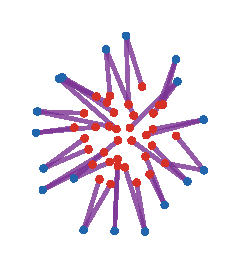
\includegraphics[width=.30\linewidth]{figures/matching-resolution-and-weights/rectangular.pdf} &
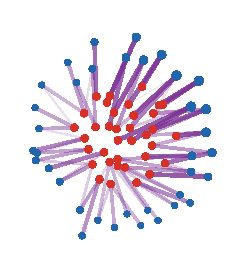
\includegraphics[width=.30\linewidth]{figures/matching-resolution-and-weights/weighted.pdf} \\[-.1em]
\small $n=m$ &
\small $m<n$ &
\small $n=m$ but $\b_j\neq 1/n$
\end{tabular}
\caption{\emph{From assignments to transport plans, using the same disk-to-annulus geometry as Figure~\ref{fig:matching-2d-cost-exponent}.} In the balanced equal-weight case, each source atom is matched to one target atom. With a target cloud that has half as many atoms, or with strongly nonuniform target weights, the coupling matrix can merge or split mass; segment thickness and opacity encode its nonzero entries, and blue marker areas encode the prescribed target masses.}
\index{plan!transport}% strictindex
\label{fig:matching-resolution-and-weights}
\end{figure}

\begin{proposition}[Rational weights as duplicated uniform matching]\label{prop-rational-weights-duplicated-matching}
\index{rational weights}% strictindex
\index{matching!uniform}% strictindex
	Let
	\[
		\al=\sum_{i=1}^n \frac{k_i}{N}\delta_{x_i},
		\qquad
		\be=\sum_{j=1}^m \frac{\ell_j}{N}\delta_{y_j},
		\qquad
		\sum_i k_i=\sum_j\ell_j=N,
	\]
	with positive integers $k_i,\ell_j$. Replace each $x_i$ by $k_i$ identical copies and each $y_j$ by $\ell_j$ identical copies, producing two uniform $N$-point clouds. Then the duplicated assignment problem and the discrete Kantorovich problem between $\al$ and $\be$ have the same optimal value. Moreover, there exists an optimal coupling of the form
	\[
	\P_{i,j}=\frac{n_{i,j}}{N},
		\qquad
		n_{i,j}\in\NN,
		\qquad
		\sum_j n_{i,j}=k_i,
		\quad
		\sum_i n_{i,j}=\ell_j,
	\]
	and couplings whose scaled entries $N\P_{i,j}$ are integral are exactly the collapsed assignments between duplicated clouds. Fractional optimal couplings may nevertheless coexist when the optimum is degenerate.
\index{Kantorovich!problem}% strictindex
\index{optimal coupling}% strictindex
\index{assignment problem}% strictindex
\end{proposition}
\begin{proof}
Any assignment between the duplicated source and target clouds defines integers $n_{i,j}$ counting how many copied particles of type $x_i$ are matched to copied particles of type $y_j$. These counts satisfy $\sum_j n_{i,j}=k_i$ and $\sum_i n_{i,j}=\ell_j$, and the associated coupling $\P_{i,j}=n_{i,j}/N$ has marginals $k_i/N$ and $\ell_j/N$. The assignment cost is $\frac1N\sum_{i,j} n_{i,j}c(x_i,y_j)=\sum_{i,j}\P_{i,j}c(x_i,y_j)$.
\index{cost!assignment}% strictindex
	Conversely, any nonnegative integer count matrix with those row and column sums can be realized by allocating the $k_i$ copies of each $x_i$ among the target copies according to $(n_{i,j})_j$. It remains to show that restricting to integral counts does not increase the optimum. Scale a feasible coupling by $N$ and write $\Q=N\P$. The constraints on $\Q$ have integer right-hand sides $(k_1,\ldots,k_n,\ell_1,\ldots,\ell_m)$. After multiplying the target rows by $-1$, their coefficient matrix is the oriented node-edge incidence matrix of a bipartite graph and is therefore totally unimodular. Every vertex of this transportation polytope is integral. Since a linear objective attains its minimum at a vertex, an integral optimal $\Q$ exists, proving equality of the two optimal values. The argument establishes existence, not integrality of every optimizer; convex combinations of distinct integral optima give fractional optima.
\index{total unimodularity}% strictindex
\index{transportation polytope}% strictindex
\index{assignment problem}% strictindex
\end{proof}

This network-flow integrality mechanism complements the Birkhoff--von Neumann theorem above (Theorem~\ref{thm-birkhoff-von-neumann}): in both cases, a linear transport relaxation has an optimizer represented by integer edge flows after scaling. The equal-unit-margin case specializes these flows to permutation matrices, whereas a degenerate optimal face may also contain fractional couplings.

Figure~\ref{fig:matching-rational-duplication} makes this reduction explicit by replacing each rational mass with identical unit copies and then regrouping the resulting uniform assignment.

\begin{figure}[H]
\centering
\begin{tabular}{ccc}
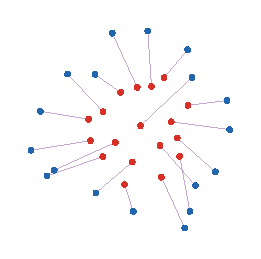
\includegraphics[width=.30\linewidth]{figures/matching-rational-duplication/uniform.pdf} &
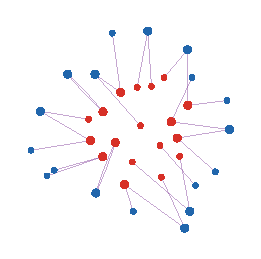
\includegraphics[width=.30\linewidth]{figures/matching-rational-duplication/binary.pdf} &
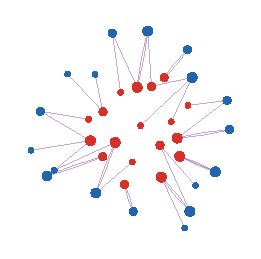
\includegraphics[width=.30\linewidth]{figures/matching-rational-duplication/ternary.pdf} \\[-.1em]
\small $k_i=\ell_j=1$ &
\small $k_i,\ell_j\in\{1,2\}$ &
\small $k_i,\ell_j\in\{1,2,3\}$
\end{tabular}
\caption{\emph{Rational weights as duplicated uniform matchings, using the same disk-to-annulus geometry as Figure~\ref{fig:matching-resolution-and-weights} with fewer displayed atoms.} The red and blue locations are kept fixed, while disk areas encode the integer multiplicities $k_i$ and $\ell_j$. Solving the assignment problem after duplicating particles produces several collapsed segments attached to high-multiplicity atoms; this is the integer count matrix of Proposition~\ref{prop-rational-weights-duplicated-matching}.}
\index{integer multiplicity}% strictindex
\index{assignment problem}% strictindex
\index{rational weights}% strictindex
\index{matching!uniform}% strictindex
\label{fig:matching-rational-duplication}
\end{figure}

\paragraph{Applications of discrete transport.}

Discrete Kantorovich transport applies whenever weighted data points or histograms must be compared through a geometry-aware correspondence. The following examples illustrate information transfer between datasets, comparison of visual distributions, and inference of temporal relations between cell populations.

\begin{example}[Application to domain adaptation]\label{ex-domain-adaptation}
\index{domain adaptation}% strictindex
\index{transfer learning}% strictindex
	In unsupervised domain adaptation, labeled source samples \((x_i^s,y_i^s)_i\) and unlabeled target samples \((x_j^t)_j\) define empirical laws $\al_s=\sum_i a_i\de_{x_i^s}$ and $\al_t=\sum_j b_j\de_{x_j^t}$.
	Writing \(\a=(a_i)_i\) and \(\b=(b_j)_j\), a Kantorovich coupling \(\P\in\CouplingsD(\a,\b)\) gives soft correspondences between the two clouds. For $b_j>0$, disintegrating $\P$ with respect to its target marginal and averaging the source labels gives the backward barycentric rule $\widetilde y_j=b_j^{-1}\sum_i \P_{i,j}y_i^s$, for either real-valued labels or one-hot class vectors. This is the label-space analogue of the barycentric projection introduced later in Definition~\ref{def-barycentric-projection}. Alternatively, the transport can be optimized jointly with a classifier by adding label-prediction terms to the feature cost. This is the mechanism behind OT domain adaptation and JDOT: the plan is not only a distance certificate, but an explicit cross-domain alignment~\cite{courty2017optimal,courty2017joint}. Learning or adapting the ground cost is the inverse viewpoint developed later in Section~\ref{sec-metric-learning-inverse-ot}.
\end{example}

\begin{example}[Application to visual distributions]\label{ex-visual-distributions}
\index{computer vision}% strictindex
\index{earth mover's distance}% strictindex
	Images, color histograms, texture descriptors and shape samples can all be represented as discrete measures. The ground cost then encodes color differences, image-plane displacements or surface distances. This viewpoint underlies the Earth Mover's Distance for image retrieval~\cite{RubTomGui00}, regularized transport for imaging~\cite{2014-xia-siims}, convolutional transport on geometric domains~\cite{2015-solomon-siggraph}, and Wasserstein barycenters for texture mixing or Radon-domain image processing~\cite{2013-Bonneel-barycenter,bonneel2023survey}. The practical gain is that the discrepancy respects geometry: moving a small amount of mass to a nearby color or pixel is cheaper than moving it far away.
\end{example}

\begin{example}[Application to single-cell population dynamics]\label{ex-cell-population-distance}\label{ex-single-cell-trajectory-inference}
\index{single-cell genomics}% strictindex
\index{trajectory inference}% strictindex
\index{Waddington-OT}% strictindex
	Single-cell sequencing observes different cells at each collection time. If \(x_i^{[k]}\in\Xx\) denotes the state of cell \(i\) at time \(t_k\), write
	\[
		\al_{t_k}=\sum_{i=1}^{n_k}a_i^{[k]}\de_{x_i^{[k]}}
		\qandq
		\a^{[k]}=(a_i^{[k]})_{i=1}^{n_k}\in\simplex_{n_k}.
	\]
	Thus a cell is one atom of an empirical population measure, rather than itself a measure over genes as in Example~\ref{ex-gene-expression-distance}. A balanced transport between two consecutive snapshots is represented by a matrix \(\P^{[k]}\in\RR_+^{n_k\times n_{k+1}}\) satisfying
	\[
		\P^{[k]}\ones_{n_{k+1}}=\a^{[k]}
		\qandq
		(\P^{[k]})^\top\ones_{n_k}=\a^{[k+1]}.
	\]
	Its entry \(\P^{[k]}_{i,j}\) is a soft ancestor--descendant mass, not evidence that the same cell was observed twice. For every row with positive sum, the normalization
	\[
		\K^{[k]}_{i,j}
		\eqdef
		\frac{\P^{[k]}_{i,j}}{\sum_{j'=1}^{n_{k+1}}\P^{[k]}_{i,j'}}
	\]
	defines a conditional transition probability; multiplying successive matrices \(\K^{[k]}\) yields population-level lineage probabilities across several collection times.

	Waddington-OT modifies this balanced baseline by incorporating growth estimates and relaxing the marginal constraints through unbalanced transport, as discussed in Example~\ref{ex-unbalanced-single-cell}~\cite{schiebinger2017reconstruction}. Related continuous and entropic constructions include trajectory inference and generative transport models~\cite{TongHuangWolfVanDijkKrishnaswamy2020TrajectoryNet,LavenantZhangKimSchiebinger2021TrajectoryInference,KleinUsciddaTheisCuturi2023GENOT}. Figure~\ref{fig:kantorovich-waddington-ot} displays three observed population snapshots in the common force-layout embedding used by Waddington-OT; this visualization need not coincide with the ground geometry used to compute \(\P^{[k]}\).
\end{example}

\begin{figure}[htbp]
\centering
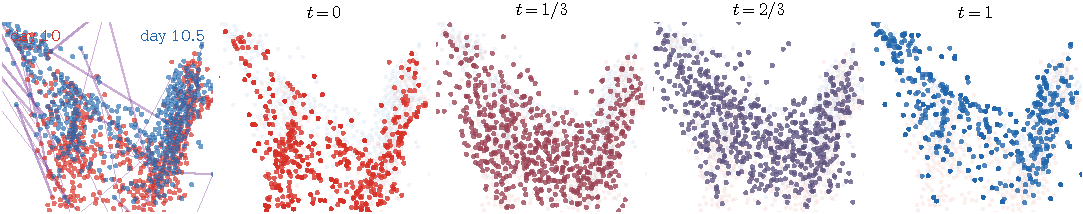
\includegraphics[width=.98\linewidth]{figures/kantorovich-waddington-ot/waddington-ot.pdf}
\caption{\emph{Three snapshots of the Waddington-OT single-cell reprogramming time course.} The first panel aggregates a representative sample from all collection times and colors cells from red to blue according to time. The remaining panels highlight the populations observed at days \(0\), \(9\), and \(18\), while cells from other times remain in gray. Every panel uses the same official force-layout embedding and viewport; no transport coupling or interpolated trajectory is displayed.}
\index{single-cell genomics}% strictindex
\index{trajectory inference}% strictindex
\label{fig:kantorovich-waddington-ot}
\end{figure}

%%%%%%%%%%%%%%%%%%%%%%%%%%%%%%%%%%%%%%%%%%%%%%%%%%%%%%%%%%%%%%%%%%%%%%%%%%%
\section{Linear-Programming Algorithms}
\index{linear!programming}% strictindex
\label{sec-kantorovich-lp-algorithms}

The discrete Kantorovich problem is a linear program with much more structure than a generic dense LP. Its variables are the arcs of a complete bipartite network, its equality constraints are flow-conservation constraints, and its extreme points are sparse tree-like couplings. This is why classical transportation algorithms remain important even though the formulation is finite-dimensional and convex.
\index{Kantorovich!problem}% strictindex
\index{equality constraint}% strictindex
\index{flow!conservation}% strictindex
\index{extreme point}% strictindex

\paragraph{Transportation simplex and network simplex.}
\index{transportation simplex}% strictindex
\index{simplex network}% strictindex

The transportation simplex goes back to Dantzig's formulation of the transportation problem~\cite{Dantzig51}. It works on basic feasible couplings, whose positive support is completed into a spanning tree of the bipartite supply-demand graph. Starting from a basis, for instance one produced by the north-west corner rule, reduced costs identify whether an unused arc can decrease the objective. Adding such an arc creates a unique cycle in the tree; one then pushes as much mass as possible around this cycle and removes the exhausted arc. This is exactly the simplex method specialized to the transportation polytope, with pivots that can be implemented using graph operations instead of a generic basis inverse.
\index{spanning tree}% strictindex
\index{feasible coupling}% strictindex
\index{north-west corner!rule}% strictindex
\index{transportation polytope}% strictindex
\index{cost!reduced}% strictindex

The network simplex is the corresponding pivoting method for general minimum-cost-flow problems~\cite{bertsekas1988dual}. It keeps node potentials, reduced costs and a spanning-tree basis, and it has become one of the most effective exact solvers for medium-scale discrete OT. Like the ordinary simplex method, its worst-case number of pivots can be exponential for adversarial instances, but the per-pivot operations exploit sparsity and are very efficient in practice. For theoretical polynomial guarantees, one can instead use strongly polynomial minimum-cost-flow algorithms, such as Orlin's algorithm~\cite{Orlin1997}. In a dense balanced transportation problem with $n$ sources and $n$ targets, the graph has $O(n)$ vertices and $O(n^2)$ arcs, so these general bounds are polynomial but still much heavier than the nearly matrix-vector structure that Sinkhorn will exploit.
\index{flow!minimum-cost}% strictindex
\index{simplex network}% strictindex

\paragraph{Interior-point methods.}
\index{interior-point method}% strictindex

Generic interior-point methods approach the same LP through a smooth central path. Assume here that all entries of $\a$ and $\b$ are positive; zero-mass rows and columns must first be removed. The logarithmic-barrier problem on the resulting transport polytope is
\index{barrier!logarithmic}% strictindex
\index{transportation polytope}% strictindex
\index{central path}% strictindex
\eql{\label{eq-transport-log-barrier}
	\P_\epsilon
	\eqdef
	\uargmin{\substack{\P\ones_m=\a,\ \P^\top\ones_n=\b\\ \P_{i,j}>0}}
		\dotp{\C}{\P}
		-
		\epsilon\sum_{i,j}\log \P_{i,j},
}
where $\epsilon>0$ is decreased along the algorithm. The barrier is singular at the boundary, so each iterate stays strictly inside the transportation polytope; as $\epsilon\downarrow0$, the central path approaches the set of LP minimizers. Each Newton step solves a linear system involving the marginal constraints and the current diagonal Hessian $\operatorname{diag}(\epsilon/\P_{i,j}^2)$, which gives robust polynomial complexity but can be expensive for dense couplings~\cite{nesterov1994interior}.
\index{Newton step}% strictindex
\index{transportation polytope}% strictindex
\index{marginal!constraint}% strictindex
\index{central path}% strictindex

Figure~\ref{fig:kantorovich-log-barrier-lp-geometry} isolates this mechanism on a two-dimensional polytope: decreasing the barrier parameter moves the minimizer along the central path toward the optimal face.

\begin{figure}[H]
\centering
\setlength{\tabcolsep}{2pt}
\begin{tabular}{@{}cccc@{}}
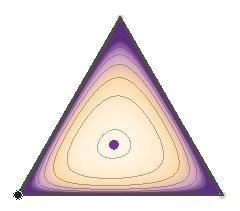
\includegraphics[width=.21\linewidth]{figures/kantorovich-log-barrier-lp-geometry/barrier-large.pdf} &
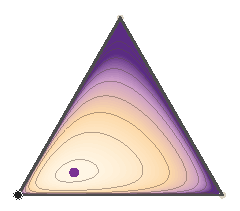
\includegraphics[width=.21\linewidth]{figures/kantorovich-log-barrier-lp-geometry/barrier-medium.pdf} &
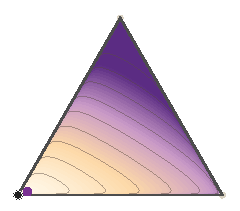
\includegraphics[width=.21\linewidth]{figures/kantorovich-log-barrier-lp-geometry/barrier-small.pdf} &
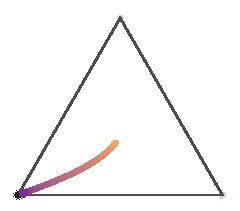
\includegraphics[width=.21\linewidth]{figures/kantorovich-log-barrier-lp-geometry/barrier-path.pdf} \\[-.1em]
\small large $\epsilon$ &
\small medium $\epsilon$ &
\small small $\epsilon$ &
\small central path
\index{central path}% strictindex
\end{tabular}
\caption{\emph{Logarithmic-barrier central path for a two-dimensional equilateral triangular slice of a linear program.} The first three panels display level sets of $\ell^\top z-\epsilon\sum_i\log(b_i-\dotp{a_i}{z})$ for decreasing barrier strengths. The last panel removes the objective background and shows only the central path inside the feasible triangle. Large $\epsilon$ selects a central interior point; decreasing $\epsilon$ moves the minimizer toward the optimal vertex while never touching the boundary. This should be contrasted with entropic OT, where the entropy temperature $\epsilon$ is usually fixed and defines the regularized problem itself.}
\index{barrier!logarithmic}% strictindex
\label{fig:kantorovich-log-barrier-lp-geometry}
\end{figure}

The comparison with Sinkhorn is therefore subtle. Both methods keep iterates positive, but they use positivity in different ways. Interior-point algorithms solve the original LP by decreasing the barrier parameter $\epsilon$ and following a central path. Sinkhorn fixes an entropic temperature $\epsilon$ and solves a different, KL-regularized OT problem by alternating diagonal scalings. The parameter $\epsilon$ may be decreased in continuation strategies, but for a fixed run it is part of the objective rather than only an algorithmic barrier.
\index{barrier!parameter}% strictindex
\index{central path}% strictindex

%%%%%%%%%%%%%%%%%%%%%%%%%%%%%%%%%%%%%%%%%%%%%%%%%%%%%%%%%%%%%%%%%%%%%%%%%%%
\section{Relaxation for Arbitrary Measures}
\index{Kantorovich!relaxation}% strictindex
\label{sec-kantorovich-continuous}

This section lifts the finite-dimensional coupling matrix to a joint probability measure. The payoff is that existence, duality and metric properties can be stated for arbitrary laws, including discrete, singular and continuous distributions.
\index{probability measure}% strictindex

\paragraph{Continuous couplings.}
\index{continuous!coupling}% strictindex

The first step is to formalize what it means for a joint law to have prescribed marginals.
\index{joint!law}% strictindex

\begin{defn}[Marginals of a joint measure]\label{def-joint-marginals}
\index{joint!measure}% strictindex
	Let $\pi\in\Mm_+^1(\Xx\times\Yy)$ and let $P_\Xx(x,y)=x$, $P_\Yy(x,y)=y$ be the coordinate projections. The marginals of $\pi$ are
	\[
		\pi_1\eqdef(P_\Xx)_\sharp\pi\in\Mm_+^1(\Xx),
		\qquad
		\pi_2\eqdef(P_\Yy)_\sharp\pi\in\Mm_+^1(\Yy).
	\]
	Equivalently, for all bounded continuous test functions $f$ on $\Xx$ and $g$ on $\Yy$,
	\[
		\int_{\Xx\times\Yy} f(x)\d\pi(x,y)=\int_\Xx f\d\pi_1,
		\qquad
		\int_{\Xx\times\Yy} g(y)\d\pi(x,y)=\int_\Yy g\d\pi_2.
	\]
\end{defn}

A useful mnemonic for the marginal constraint $\pi_1=\al$ and $\pi_2=\be$ is the formal row-and-column notation
\index{marginal!constraint}% strictindex
\[
	\int_\Yy \d\pi(x,y)=\d\al(x),
	\qquad
	\int_\Xx \d\pi(x,y)=\d\be(y),
\]
which is made rigorous by Definition~\ref{def-joint-marginals}, or equivalently by the identities $\pi(A\times\Yy)=\al(A)$ and $\pi(\Xx\times B)=\be(B)$ for measurable sets $A\subset\Xx$ and $B\subset\Yy$.

\begin{defn}[Couplings]\label{def-continuous-couplings}
\index{continuous!coupling}% strictindex
	Given $\al\in\Mm_+^1(\Xx)$ and $\be\in\Mm_+^1(\Yy)$, the set of couplings between $\al$ and $\be$ is
	\eql{\label{eq-coupling-generic}
		\Couplings(\al,\be)
		\eqdef
		\enscond{\pi\in\Mm_+^1(\Xx\times\Yy)}{\pi_1=\al \qandq \pi_2=\be}.
	}
	This is the continuous analogue of the transportation polytope~\eqref{eq-discr-couplings}.
\index{transportation polytope}% strictindex
\end{defn}

\begin{rem}[Probabilistic interpretation of couplings]
	If $X\sim\al$ and $Y\sim\be$, then $\pi\in\Couplings(\al,\be)$ means that $\pi$ is the law of a pair $(X,Y)$ whose coordinates have laws $\al$ and $\be$. The coupling encodes the dependence between $X$ and $Y$. The tensor product $\al\otimes\be$ corresponds to independence, whereas a graph coupling $(\Id,T)_\sharp\al$ corresponds to the deterministic relation $Y=T(X)$.

	In the discrete case, when $\al=\sum_i \a_i\de_{x_i}$ and $\be=\sum_j \b_j\de_{y_j}$, the constraint $\pi_1=\al$ and $\pi_2=\be$ forces every coupling to have the form $\pi=\sum_{i,j}\P_{i,j}\de_{(x_i,y_j)}$ with $\P\in\CouplingsD(\a,\b)$. The discrete formulation is therefore a special case of the continuous one, not merely an approximation.
\end{rem}

Unlike the Monge constraint, the coupling constraint is never empty. The continuous feasibility witness is the tensor product coupling, the measure-theoretic version of the discrete product plan above.

\begin{defn}[Tensor product and trivial coupling]\label{def-tensor-product-coupling}
\index{product!coupling}% strictindex
\index{tensor product coupling}% strictindex
	Given $\al\in\Mm_+^1(\Xx)$ and $\be\in\Mm_+^1(\Yy)$, the tensor product coupling $\al\otimes\be$ is the probability measure on $\Xx\times\Yy$ defined by
	\[
		\int_{\Xx\times\Yy} h(x,y)\d(\al\otimes\be)(x,y)
		=
		\int_\Xx\left(\int_\Yy h(x,y)\d\be(y)\right)\d\al(x)
	\]
	for every bounded measurable $h$. It is also called the trivial coupling because it makes the two coordinates independent.
\end{defn}
Indeed, for every $f\in\Cc_b(\Xx)$,
\[
	\int_{\Xx\times\Yy} f(x)\d(\al\otimes\be)(x,y)
	=
	\left(\int_\Xx f(x)\d\al(x)\right)\left(\int_\Yy\d\be(y)\right)
	=
	\int f\d\al,
\]
and similarly for the second marginal, so $\al\otimes\be\in\Couplings(\al,\be)$.

The next result echoes Proposition~\ref{prop-discrete-product-coupling-degenerate} in the continuous setting. In both cases, the independent coupling is optimal precisely when the objective is flat over the whole admissible set; for continuous costs, this flatness is equivalently the additive form $c(x,y)=u(x)+v(y)$ on the product support.

\begin{prop}[Product optimality is degenerate]\label{prop-product-coupling-degenerate}
\index{product!coupling}% strictindex
	Assume that $\Xx$ and $\Yy$ are compact metric spaces and that $c\in\Cc(\Xx\times\Yy)$. The following statements are equivalent:
	\[
		\al\otimes\be\in\uargmin{\pi\in\Couplings(\al,\be)}\int c\,\d\pi,
		\qquad
		\text{every coupling in }\Couplings(\al,\be)\text{ is optimal}.
	\]
	They are also equivalent to the additive decomposition of the cost on the product support,
	\[
		c(x,y)=u(x)+v(y),
		\qquad
		u\in\Cc(\supp(\al)),\quad v\in\Cc(\supp(\be)).
	\]
\end{prop}
\begin{proof}
	If every coupling is optimal, then $\al\otimes\be$ is optimal. Conversely, assume that $\al\otimes\be$ is optimal. We first show that, for every $x_0,x_1\in\supp(\al)$ and $y_0,y_1\in\supp(\be)$,
	\[
		c(x_0,y_0)+c(x_1,y_1)
		=
		c(x_0,y_1)+c(x_1,y_0).
	\]
	Indeed, if this equality failed, after exchanging $y_0$ and $y_1$ if necessary one would have a strict inequality
	\[
		c(x_0,y_0)+c(x_1,y_1)
		>
		c(x_0,y_1)+c(x_1,y_0).
	\]
		Failure of the equality forces $x_0\neq x_1$ and $y_0\neq y_1$. By continuity, the strict inequality persists with a uniform margin on small neighborhoods $U_0,U_1$ of $x_0,x_1$ and $V_0,V_1$ of $y_0,y_1$, chosen disjoint within each pair. Since the four points lie in the supports, these neighborhoods have positive marginal mass. Denote by $\al_i$ and $\be_i$ the normalized restrictions of $\al$ to $U_i$ and of $\be$ to $V_i$, and choose
	\[
		0<\lambda\leq
		\min\{\al(U_0)\be(V_0),\al(U_1)\be(V_1)\}.
	\]
	The exchanged measure
	\[
		\tilde\pi
		=
		\al\otimes\be
		-\lambda\,\al_0\otimes\be_0
		-\lambda\,\al_1\otimes\be_1
		+\lambda\,\al_0\otimes\be_1
		+\lambda\,\al_1\otimes\be_0
	\]
	is nonnegative and has the same two marginals as $\al\otimes\be$. The uniform strict inequality on the neighborhoods implies that $\int c\,\d\tilde\pi<\int c\,\d(\al\otimes\be)$, contradicting optimality.

	Fixing any $x_\star\in\supp(\al)$ and $y_\star\in\supp(\be)$, the equality of cross differences gives, for all $(x,y)\in\supp(\al)\times\supp(\be)$,
	\[
		c(x,y)=c(x,y_\star)+c(x_\star,y)-c(x_\star,y_\star).
	\]
		Thus $c=u+v$ on the product support, with $u(x)=c(x,y_\star)-c(x_\star,y_\star)$ and $v(y)=c(x_\star,y)$. These functions are continuous on the corresponding supports. Every coupling is concentrated on this product support, so for any $\pi\in\Couplings(\al,\be)$,
	\(\int c\,\d\pi = \int u\,\d\al+\int v\,\d\be\),
	which depends only on the marginals. Hence all couplings are optimal.
\end{proof}

The tensor product is therefore a trivial feasible coupling, not a typical optimizer. Product optimality means that the cost cannot distinguish between dependences once the marginals are fixed. The continuity assumption is important: if $\al=\be$ is the uniform law on $[0,1]$ and $c(x,y)=\ones_{\{x=y\}}$, then $\al\otimes\be$ has zero cost and is optimal, whereas the identity coupling has cost one. Thus, for arbitrary merely measurable costs, changing the cost on an $\al\otimes\be$-negligible set may affect singular couplings without changing the product cost.
\index{feasible coupling}% strictindex

If there exists a map $T:\Xx\to\Yy$ such that $T_\sharp\al=\be$, then the Monge map induces the graph coupling $\pi=(\Id,T)_\sharp\al\in\Couplings(\al,\be)$, characterized by
\index{Monge!problem}% strictindex
\[
	\int_{\Xx\times\Yy} h(x,y)\d\pi(x,y)
	=
	\int_\Xx h(x,T(x))\d\al(x).
\]
Applying this identity to $h(x,y)=f(x)$ or $h(x,y)=g(y)$ gives respectively $\pi_1=\al$ and $\pi_2=\be$. Thus graph couplings are precisely the Kantorovich representation of deterministic Monge maps.
A last important class consists of semi-discrete problems, where $\al$ has a density and $\be$ is discrete. Every coupling is then supported on the union of the slices $\Xx\times\{y_j\}$. When an optimal coupling is induced by a map, these slices are selected by a partition of $\Xx$ into transport cells, as developed in Chapter~\ref{sec-semidiscr-w1}.
\index{semi-discrete!OT}% strictindex

\begin{rem}[Book-shifting as a flat Kantorovich face]\label{rem-kantorovich-book-shifting}
\index{book-shifting}% strictindex
\index{Wasserstein!W1 non-uniqueness}% strictindex
	The Monge book-shifting example in Example~\ref{ex-monge-book-shifting-w1} has a transparent coupling interpretation. Let $\al$ be uniform on $[0,2]$ and $\be$ uniform on $[1,3]$. For every $\pi\in\Couplings(\al,\be)$,
	\[
		\int |y-x|\d\pi(x,y)
		\geq
		\int (y-x)\d\pi(x,y)
		=
		\int y\d\be(y)-\int x\d\al(x)
		=1.
	\]
	Equality holds exactly for couplings concentrated on the half-plane $\{(x,y):y\geq x\}$, where $|y-x|=y-x$. Hence the optimal set is a whole face of the coupling polytope, not a single graph. The translation and book-shifting maps give two graph couplings inside this face, but many non-deterministic couplings are optimal as well.
\index{graph!coupling}% strictindex
\index{optimal coupling}% strictindex
\end{rem}

\paragraph{Continuous Kantorovich problem.}
\index{Kantorovich!problem}% strictindex

The discrete Kantorovich relaxation of Section~\ref{sec-discrete-relaxation}, formalized in Definition~\ref{def-discrete-kantorovich-problem}, extends from nonnegative coupling matrices to coupling measures between arbitrary probability measures.
\begin{defn}[Continuous Kantorovich problem]\label{def-continuous-kantorovich-problem}
For $\al\in\Mm_+^1(\Xx)$, $\be\in\Mm_+^1(\Yy)$, and a nonnegative Borel cost $c:\Xx\times\Yy\to[0,+\infty]$, define
\eql{\label{eq-mk-generic}
	\MK_c(\al,\be)
	\eqdef
	\inf_{\pi\in\Couplings(\al,\be)}
	\int_{\Xx\times\Yy} c(x,y)\d\pi(x,y).
}
A minimizer is an optimal coupling, or optimal transport plan.
The value is understood in $[0,+\infty]$.
\end{defn}
This is an infinite-dimensional linear program over a space of measures.
\index{infinite-dimensional linear programming}% strictindex

The following result generalizes Proposition~\ref{prop-discrete-kantorovich-joint-convexity} from coupling matrices to coupling measures: the Kantorovich value is convex in the marginals but concave in the ground cost.

\begin{prop}[Convexity in the marginals and concavity in the cost]\label{prop-kantorovich-value-curvature}
\index{cost!transport}% strictindex
\index{convexity!Kantorovich value}% strictindex
\index{concavity!Kantorovich value}% strictindex
	Fix a nonnegative Borel cost $c$. The extended-valued map
	\[
		(\al,\be)\longmapsto\MK_c(\al,\be)
	\]
	is jointly convex on pairs of probability measures. Conversely, for fixed marginals $(\al,\be)$, the map $c\mapsto\MK_c(\al,\be)$ is concave on the cone of nonnegative Borel costs: for any such $c_0,c_1$ and $t\in[0,1]$,
	\[
		\MK_{(1-t)c_0+tc_1}(\al,\be)
		\geq
		(1-t)\MK_{c_0}(\al,\be)+t\MK_{c_1}(\al,\be).
	\]
	The inequality is understood in $[0,+\infty]$; in particular, the map is concave on every convex family of costs on which it is finite.
\end{prop}

\begin{proof}
	For joint convexity, let $(\al_0,\be_0)$ and $(\al_1,\be_1)$ be two pairs of probability measures. The claim is immediate at $t\in\{0,1\}$ or if one of the two values on the right-hand side is infinite. Otherwise, for $\eta>0$, choose $\pi_i\in\Couplings(\al_i,\be_i)$ such that $\int c\d\pi_i\leq\MK_c(\al_i,\be_i)+\eta$ for $i\in\{0,1\}$.
	Then $(1-t)\pi_0+t\pi_1$ couples $(1-t)\al_0+t\al_1$ and $(1-t)\be_0+t\be_1$, and hence
	\[
		\MK_c\big((1-t)\al_0+t\al_1,(1-t)\be_0+t\be_1\big)
		\leq
		(1-t)\MK_c(\al_0,\be_0)+t\MK_c(\al_1,\be_1)+\eta.
	\]
	Letting $\eta\to0$ proves joint convexity.

	For concavity, the endpoint cases are immediate, so assume $t\in(0,1)$ and fix $\pi\in\Couplings(\al,\be)$. Linearity of integration for nonnegative functions gives
	\[
		\int\big((1-t)c_0+tc_1\big)\d\pi
		\geq
		(1-t)\MK_{c_0}(\al,\be)+t\MK_{c_1}(\al,\be).
	\]
	Taking the infimum over $\pi$ proves the stated inequality.
\end{proof}

\begin{rem}[Probabilistic interpretation of Kantorovich's problem]
	The continuous Kantorovich problem of Definition~\ref{def-continuous-kantorovich-problem} can equivalently be written as
	\[
		\MK_c(\al,\be)
		=
		\inf_{X\sim\al,\,Y\sim\be}\EE(c(X,Y)).
	\]
	The minimization is not over the marginal laws, which are fixed, but over all possible dependences between the two random variables. OT therefore chooses the cheapest joint law among all couplings.
\index{random variable}% strictindex
\index{joint!law}% strictindex
\end{rem}

Existence is one of the decisive gains of Kantorovich relaxation. The Monge problem of Definition~\ref{def-monge-problem} may have no admissible map, and even when maps exist its infimum need not be attained because graph couplings are not closed under weak limits. By contrast, $\Couplings(\al,\be)$ always contains the product coupling $\al\otimes\be$; tightness and weak closedness then make the direct method available.

\begin{prop}[Existence for lower-semicontinuous costs]\label{prop-kantorovich-existence-compact}
\index{lower semicontinuity}% strictindex
		Assume that $\Xx$ and $\Yy$ are Polish spaces and that $c:\Xx\times\Yy\to[0,+\infty]$ is lower semicontinuous. Then the Kantorovich problem~\eqref{eq-mk-generic} admits at least one minimizer. In particular, this applies to every continuous nonnegative cost on compact metric spaces.
\index{Kantorovich!problem}% strictindex
\end{prop}
\begin{proof}
		The constraint set is non-empty because it contains the product coupling $\al\otimes\be$. It is uniformly tight: given $\varepsilon>0$, choose compact sets $K_\Xx\subset\Xx$ and $K_\Yy\subset\Yy$ such that $\al(K_\Xx)\geq1-\varepsilon/2$ and $\be(K_\Yy)\geq1-\varepsilon/2$. Every $\pi\in\Couplings(\al,\be)$ then satisfies
		\(\pi(K_\Xx\times K_\Yy)\geq1-\varepsilon\).
		By Prokhorov's theorem~\cite{bogachev2007measure,Villani09}, the set of couplings is relatively compact for weak convergence; the weak topology is reviewed in Section~\ref{sec-wasserstein-topology-applications}. It is also weakly closed, because the coordinate projections are continuous and therefore preserve the marginal identities in the limit. Hence $\Couplings(\al,\be)$ is weakly compact. Finally, Portmanteau's theorem makes $\pi\mapsto\int c\d\pi$ weakly lower semicontinuous. The direct method gives a minimizer.
\index{Prokhorov theorem}% strictindex
\index{Portmanteau theorem}% strictindex
\index{probability measure}% strictindex
\index{marginal!constraint}% strictindex
\index{product!coupling}% strictindex
\index{weak!convergence}% strictindex
\index{topology!weak}% strictindex
\end{proof}

\paragraph{Axiomatic characterization of the relaxation.}
\index{Kantorovich!axiomatic characterization}% strictindex
\index{convex envelope!Kantorovich cost}% strictindex

Kantorovich relaxation is not only a convenient enlargement of Monge's problem: convexity and weak stability single it out as the maximal extension of the pointwise ground cost from pairs of points to pairs of probability measures.

\begin{thm}[Kantorovich cost as the maximal convex relaxation]\label{thm-kantorovich-maximal-convex-relaxation}
	Assume that $\Xx$ and $\Yy$ are compact metric spaces and that $c:\Xx\times\Yy\to[0,+\infty)$ is continuous. Then $\MK_c$ is the pointwise largest proper functional
	\[
		\mathsf F:\Mm_+^1(\Xx)\times\Mm_+^1(\Yy)\longrightarrow(-\infty,+\infty]
	\]
	that is jointly convex, weakly lower semicontinuous, and satisfies
	\[
		\mathsf F(\de_x,\de_y)\leq c(x,y)
		\qquad\text{for every }(x,y)\in\Xx\times\Yy.
	\]
	More precisely, every such $\mathsf F$ satisfies $\mathsf F(\al,\be)\leq\MK_c(\al,\be)$ for all $(\al,\be)$,
	while $\MK_c$ itself has these properties and obeys $\MK_c(\de_x,\de_y)=c(x,y)$.
\end{thm}
\begin{proof}
	Joint convexity follows from Proposition~\ref{prop-kantorovich-value-curvature}. For weak lower semicontinuity, consider converging marginals and optimal plans along a subsequence realizing the lower limit. Compactness gives a further weakly convergent subsequence; its limit has the limiting marginals, and lower semicontinuity of the integral gives the claim, exactly as in Proposition~\ref{prop-kantorovich-existence-compact}. The only coupling of $(\de_x,\de_y)$ is $\de_{(x,y)}$, which proves the identity on Dirac pairs.

	Fix $\pi\in\Couplings(\al,\be)$. Its marginal constraints are exactly the barycentric identity $(\al,\be)=\int(\de_x,\de_y)\d\pi$.
	Jensen's inequality for lower-semicontinuous convex functionals therefore gives
	\[
		\mathsf F(\al,\be)
		\leq\int\mathsf F(\de_x,\de_y)\d\pi(x,y)
		\leq\int c(x,y)\d\pi(x,y).
	\]
	Taking the infimum over $\pi\in\Couplings(\al,\be)$ proves maximality.
\end{proof}

This is the probability-measure specialization of the convex-envelope theorem of Savar\'e and Sodini~\cite[Theorem~4.4]{SavareSodini2022}, which treats finite measures on completely regular spaces. The word \emph{largest} is essential: joint convexity, weak lower semicontinuity and equality on Dirac pairs only imply that another extension lies below $\MK_c$; they do not force it to coincide with $\MK_c$.

\paragraph{Monge--Kantorovich equivalence.}
\index{Monge-Kantorovich equivalence}% strictindex

The proof of Brenier's theorem~\ref{thm-brenier} relies on Kantorovich relaxation and duality. It proves that, under its hypotheses, the relaxation is tight: it has the same cost as the Monge problem and its optimal coupling is induced by a map.
\index{optimal coupling}% strictindex
\index{Brenier!theorem}% strictindex
\index{Kantorovich!relaxation}% strictindex
\index{Monge!problem}% strictindex

\begin{cor}[Monge--Kantorovich equivalence under Brenier]\label{cor-monge-kantorovich-brenier}
\index{Monge-Kantorovich equivalence}% strictindex
		Let $\al,\be\in\Pp_2(\RR^d)$, assume that $\al$ is absolutely continuous with respect to Lebesgue measure, and let $c(x,y)=\norm{x-y}^2$. If $T$ is the Brenier map solving Monge's problem, then $\pi=(\Id,T)_\sharp\al$ is the unique optimal coupling solving the Kantorovich problem. In particular, Monge and Kantorovich costs are the same.
\index{Lebesgue measure}% strictindex
\index{Kantorovich!problem}% strictindex
\index{optimal coupling}% strictindex
\index{Brenier!map}% strictindex
\end{cor}
\begin{proof}
	The proof of Brenier's theorem shows that the support of any optimal Kantorovich plan is contained in the subdifferential $\partial\phi$ of a convex function $\phi$. When $\al$ has a density, $\phi$ is differentiable $\al$-almost everywhere, so $\partial\phi(x)=\{\nabla\phi(x)\}$ for $\al$-almost every $x$. Thus every optimal coupling is concentrated on the graph of $T=\nabla\phi$ and must equal $(\Id,T)_\sharp\al$. The graph coupling is feasible and optimal, and the two formulations have the same value.
\index{support}% strictindex
\index{subdifferential}% strictindex
\index{convex!function}% strictindex
\index{Brenier!theorem}% strictindex
\end{proof}

The density assumption is exactly what prevents the relaxed plan from using several destinations at a nonsmooth point.

\begin{rem}[Nonsmooth potentials and splitting]
	If $\al$ does not have a density, then $\phi$ may be non-smooth on a set charged by $\al$, and non-smooth points can lead to mass splitting. For instance, moving $\delta_0$ to $(\delta_{-1}+\delta_{+1})/2$ can be represented by a plan concentrated on the set-valued subdifferential of $\phi(x)=|x|$, but not by a deterministic map. This is the continuous counterpart of the gap between the uniform matching case of Corollary~\ref{cor-kantorovich-matching} and the general splitting case.
\index{matching!uniform}% strictindex
\end{rem}

\begin{rem}[Probabilistic form of tightness]
\index{tightness}% strictindex
	If $(X,Y)$ has the optimal Kantorovich law under the assumptions of Corollary~\ref{cor-monge-kantorovich-brenier}, then $Y=T(X)$ almost surely with $X\sim\al$ and $T(X)\sim\be$. This is analogous to the Birkhoff--von Neumann result in the fully discrete uniform case: in both settings, the convex relaxation admits an optimizer satisfying the original deterministic constraint. The hypotheses are quite different, however: Birkhoff--von Neumann is finite-dimensional and need not give uniqueness, whereas Brenier's theorem uses absolute continuity of the source and gives uniqueness of the optimal map almost everywhere.
\index{Birkhoff!von Neumann theorem}% strictindex
\index{Brenier!theorem}% strictindex
\index{absolute continuity}% strictindex
\end{rem}

\phantomsection
\paragraph{Kantorovich solution in 1D.}\label{sec-1d-kantorovich-solution}
\index{Kantorovich!coupling}% strictindex
\index{quantile!coupling}% strictindex

The atomless assumption in the Monge statement of Section~\ref{sec-1d-transport-quantiles} is a limitation of maps, not of one-dimensional optimality. Once couplings are allowed, atoms can be split by assigning subintervals of quantile levels to different target points. The common quantile parameter therefore defines an optimal relaxed coupling for arbitrary probability measures.

\begin{thm}[One-dimensional Kantorovich solution]\label{prop-1d-kantorovich-quantile-coupling}
\index{monotone!rearrangement}% strictindex
\index{quantile!coupling}% strictindex
\index{Kantorovich!problem}% strictindex
		Let $\al,\be\in\Mm_+^1(\RR)$ and let $h:\RR\to[0,+\infty)$ be convex. Consider the cost $c(x,y)=h(x-y)$. Write $q_\al\eqdef\cumul{\al}^{-1}$ and $q_\be\eqdef\cumul{\be}^{-1}$, and assume that $h(q_\al-q_\be)\in L^1(0,1)$. Then the quantile coupling
	\[
		\pi^\star=(q_\al,q_\be)_\sharp\mathrm{Leb}_{[0,1]}
		=
		(\cumul{\al}^{-1},\cumul{\be}^{-1})_\sharp\mathrm{Leb}_{[0,1]}
	\]
	solves the Kantorovich problem~\eqref{eq-mk-generic} for $c(x,y)=h(x-y)$.
	In particular, $h(t)=|t|^p$ gives the usual one-dimensional optimal coupling for every $p\geq1$.
\end{thm}
\begin{proof}
	The push-forward statement $\pi^\star\in\Couplings(\al,\be)$ follows from Proposition~\ref{prop-quantile-pushforward}. It remains to prove optimality.

	The key point is the one-dimensional uncrossing inequality. If $x<x'$ and $y>y'$, set $a=x-y$, $\delta=x'-x>0$ and $\eta=y-y'>0$. Convexity of $h$ implies that increments are monotone, hence
	\[
		h(a+\eta)-h(a)
		\leq
		h(a+\delta+\eta)-h(a+\delta),
	\]
	which is exactly
	\(h(x-y)+h(x'-y') \geq h(x-y')+h(x'-y)\).
	Thus removing a crossing never increases the cost. For a finite transport matrix on two ordered grids, if $i<i'$ and $j>j'$ carry crossed masses $\P_{i,j}$ and $\P_{i',j'}$, one may move $\theta=\min(\P_{i,j},\P_{i',j'})$ units of mass from the crossed entries $(i,j)$, $(i',j')$ to the uncrossed entries $(i,j')$, $(i',j)$. The row and column sums are unchanged, and the preceding inequality shows that the cost does not increase. Repeating this elementary uncrossing step yields an ordered plan; on an ordered uniform quantile grid, this is the diagonal plan.

		For general measures, apply the same argument in quantile coordinates. Let $\pi\in\Couplings(\al,\be)$. Let $U_\al$ and $U_\be$ be uniform random variables on $(0,1)$, and denote by $K_\al(x,\d r)$ and $K_\be(y,\d s)$ regular conditional laws of $U_\al$ given $q_\al(U_\al)=x$ and of $U_\be$ given $q_\be(U_\be)=y$. Given $(X,Y)\sim\pi$, draw conditionally $R\sim K_\al(X,\cdot)$ and $S\sim K_\be(Y,\cdot)$. The law $\gamma$ of $(R,S)$ has uniform marginals and satisfies $\pi=(q_\al,q_\be)_\sharp\gamma$.

		We now justify the approximation. Let $\kappa_M(r)=\max(-M,\min(r,M))$ and set $q_{\al,M}=\kappa_M\circ q_\al$ and $q_{\be,M}=\kappa_M\circ q_\be$. These functions are bounded and nondecreasing. Approximate them almost everywhere by nondecreasing step functions $q_{\al,M}^N$ and $q_{\be,M}^N$ that are constant on the uniform intervals $I_k=((k-1)/N,k/N]$. The matrix
		\(G_{k,\ell}^N=\gamma(I_k\times I_\ell)\)
		is a coupling of the two uniform histograms. Proposition~\ref{prop-1d-weighted-sweep}, applied to the ordered step values, therefore gives
		\[
			\int_0^1 h(q_{\al,M}^N(r)-q_{\be,M}^N(r))\d r
			\leq
			\int_{(0,1)^2}h(q_{\al,M}^N(r)-q_{\be,M}^N(s))\d\gamma(r,s).
		\]
		For fixed $M$, the arguments of $h$ remain in the compact interval $[-2M,2M]$. Dominated convergence as $N\to\infty$ yields the same inequality for $q_{\al,M}$ and $q_{\be,M}$.

		Finally, $\kappa_M$ is nondecreasing and $1$-Lipschitz. Hence, for every $x,y\in\RR$, there exists $t_M(x,y)\in[0,1]$ such that
		\(\kappa_M(x)-\kappa_M(y)=t_M(x,y)(x-y)\).
		Convexity and nonnegativity imply
		\[
			h(t_M(x,y)(x-y))
			\leq
			(1-t_M(x,y))h(0)+t_M(x,y)h(x-y)
			\leq h(0)+h(x-y).
		\]
		The assumed integrability controls the diagonal term. If the cost of $\pi$ is finite, the same bound controls the right-hand side; if it is infinite, the desired comparison is immediate. Dominated convergence as $M\to\infty$ therefore gives
	\[
		\int_0^1 h(q_\al(r)-q_\be(r))\d r
		\leq
		\int h(x-y)\d\pi(x,y)
	\]
	for every $\pi\in\Couplings(\al,\be)$.
\index{optimal coupling}% strictindex
\index{convex!function}% strictindex
\end{proof}

This result is strictly more flexible than the Monge formula. If $\al$ has an atom, a map can only send that whole atom to one target point, whereas the quantile interval associated with the atom can be coupled with a nontrivial portion of $\be$. The one-dimensional Kantorovich solution therefore handles mass splitting without changing the monotone geometry.

%%%%%%%%%%%%%%%%%%%%%%%%%%%%%%%%%%%%%%%%%%%%%%%%%%%%%%%%%%%%%%%%%%%%%%%%%%%
\section{Cone of Convex Functions and Monge Gap}
\label{sec-monge-gap}
\index{Monge gap}% strictindex
\index{convex!cone of functions}% strictindex

For quadratic transport, Brenier's theorem~\ref{thm-brenier} identifies optimal maps with gradients, or more generally subgradients, of convex functions. Convex functions form a cone under addition and nonnegative scaling, but imposing this global structure directly on a learned map can be difficult. The Monge gap turns transport optimality into a variational certificate: for suitable costs it is itself convex, on the line it becomes an isotonicity penalty, and in learning problems it can be added to an ordinary regression objective.

\paragraph{Definition and optimality certificate.}

Matching an output law does not identify an optimal map: many maps can have the same push-forward while incurring different transport costs. The Monge gap of Uscidda and Cuturi~\cite{UsciddaCuturi2023} separates distributional fitting from transport optimality by comparing the graph coupling generated by a map with the best coupling having exactly the same marginals.

\begin{defn}[Monge gap]\label{def-monge-gap}
	Let $\al\in\Mm_+^1(\Xx)$, let $T:\Xx\to\Yy$ be measurable, and assume that the following costs are finite. The $c$-Monge gap of $T$ relative to $\al$ is
	\eql{\label{eq-monge-gap}
		\mathcal M_\al^c(T)
		\eqdef
		\int c(x,T(x))\d\al(x)-\MK_c(\al,T_\sharp\al).
	}
\end{defn}

The second marginal is deliberately $T_\sharp\al$: the gap tests optimality of $T$, not agreement with an externally prescribed target.

\begin{prop}[Elementary properties of the Monge gap]\label{prop-monge-gap-properties}
	Under the standing Polish-space assumptions, suppose that the relevant integrals are finite. Then $\mathcal M_\al^c(T)\geq0$, with equality if and only if $(\Id,T)_\sharp\al$ is an optimal coupling between $\al$ and $T_\sharp\al$. Moreover,
	\eql{\label{eq-monge-gap-self-coupling}
		\mathcal M_\al^c(T)
		=
		\sup_{\eta\in\Couplings(\al,\al)}
		\int\big[c(x,T(x))-c(x,T(z))\big]\d\eta(x,z).
	}
	Finally, the gap is unchanged when $c(x,y)$ is replaced by $c(x,y)+r(x)+s(y)$, provided the modified cost remains admissible and all marginal terms are integrable.
\end{prop}
\begin{proof}
	The graph plan $(\Id,T)_\sharp\al$ is feasible for $\MK_c(\al,T_\sharp\al)$, which proves nonnegativity and the equality criterion. Every $\eta\in\Couplings(\al,\al)$ induces the coupling $(x,z)\mapsto(x,T(z))$. Conversely, disintegrating $\al$ along $T$ lifts every coupling in $\Couplings(\al,T_\sharp\al)$ to such a self-coupling. Subtracting the resulting infimum from the graph cost gives~\eqref{eq-monge-gap-self-coupling}. Adding $r(x)+s(y)$ shifts both terms in~\eqref{eq-monge-gap} by $\int r\d\al+\int s\d(T_\sharp\al)$.
\end{proof}

\paragraph{Convex gaps and convex potentials.}

Formula~\eqref{eq-monge-gap-self-coupling} need not be convex in $T$: both occurrences of $T$ lie inside a generic nonlinear cost. Convexity becomes automatic when cost differences are affine in the image variable.

\begin{prop}[Convex Monge gaps for affine-difference costs]\label{prop-affine-difference-monge-gap}
\index{Monge gap!convexity}% strictindex
\index{affine-difference cost}% strictindex
	Let $\Yy\subset\RR^m$ be convex and let the nonnegative cost $c$ have the form
	\eql{\label{eq-affine-difference-cost}
		c(x,y)=a(x)+b(y)-\dotp{A(x)}{y},
	}
	where $A,T\in L^2(\al;\RR^m)$ and all displayed terms are finite. Then
	\eql{\label{eq-affine-difference-monge-gap}
		\mathcal M_\al^c(T)
		=
		\sup_{\eta\in\Couplings(\al,\al)}
		\int\dotp{A(x)}{T(z)-T(x)}\d\eta(x,z).
	}
	Consequently, $T\mapsto\mathcal M_\al^c(T)$ is convex, and it is positively homogeneous when the admissible maps take values in $\RR^m$. Moreover, $\mathcal M_\al^c(T)=0$ if and only if there is a proper lower-semicontinuous convex function $\varphi$ such that
	\eql{\label{eq-affine-difference-subgradient-characterization}
		T(x)\in\partial\varphi(A(x))
		\qquad\text{for $\al$-almost every }x.
	}
\end{prop}
\begin{proof}
	\index{subdifferential}% strictindex
	The marginal terms $a$ and $b$ cancel in~\eqref{eq-monge-gap-self-coupling}, giving~\eqref{eq-affine-difference-monge-gap}; this is a supremum of linear functionals of $T$. Next, disintegrating $\al$ along $A$ lifts every coupling between $A_\sharp\al$ and $T_\sharp\al$. Hence zero gap is equivalent to optimality of $(A,T)_\sharp\al$ for the bilinear cost $(u,y)\mapsto-\dotp{u}{y}$. Up to marginal terms, this is the quadratic cost $\frac12\norm{u-y}^2$. By Rockafellar's characterization~\cite{rockafellar2015convex}, recalled in Section~\ref{sec-cyclical-monotonicity}, its optimal plans are exactly those concentrated on the subdifferential of a proper lower-semicontinuous convex function.
\end{proof}

The class~\eqref{eq-affine-difference-cost} contains $c(x,y)=\frac12\norm{x-y}^2$, for which $A(x)=x$. It also contains the Bregman divergence of Definition~\ref{def-bregman-divergence} with $x$ as base point,
\index{Bregman!divergence}% strictindex
\[
	B_\Phi(y|x)=\Phi(y)-\Phi(x)-\dotp{\nabla\Phi(x)}{y-x},
\]
where $\Phi$ is differentiable and convex: here $a(x)=\dotp{\nabla\Phi(x)}{x}-\Phi(x)$, $b(y)=\Phi(y)$ and $A(x)=\nabla\Phi(x)$. The argument order is essential: on a full-dimensional domain, the reversed divergence $B_\Phi(x|y)$ is generally not of the form~\eqref{eq-affine-difference-cost} unless $\Phi$ is quadratic. Thus the zero-gap condition generalizes Brenier's characterization: in the quadratic case it reduces to $T(x)\in\partial\varphi(x)$ $\al$-almost everywhere, and to $T=\nabla\varphi$ when $\al$ has a density.

This cost class is also exhaustive under mild smoothness. If $\Yy$ is open and $c(x,\cdot)\in C^2(\Yy)$, then the gap is convex for every source $\al$ for which it is finite---and it is enough to test finitely supported sources---if and only if $c$ has the form~\eqref{eq-affine-difference-cost}. Indeed, for $\al=\frac12(\de_{x_0}+\de_{x_1})$, $u=T(x_0)$, $v=T(x_1)$ and $g(y)=c(x_0,y)-c(x_1,y)$, one has $\mathcal M_\al^c(T)=\frac12(g(u)-g(v))_+$. Convexity in $(u,v)$ forces $\nabla^2g=0$, so every such difference is affine.

\paragraph{One-dimensional order and isotonicity.}

On the line, the order structure gives a more explicit formula, even for convex displacement costs whose Monge gap is not itself convex.

\begin{defn}[Increasing rearrangement relative to a source]\label{def-increasing-rearrangement-map}
\index{increasing rearrangement}% strictindex
	Let $\al\in\Mm_+^1(\RR)$ be atomless and let $T:\RR\to\RR$ be measurable. The increasing rearrangement of $T$ relative to $\al$ is
	\eql{\label{eq-increasing-rearrangement-map}
		T^{\uparrow,\al}
		\eqdef
		\cumul{T_\sharp\al}^{-1}\circ\cumul{\al}.
	}
	It is the unique $\al$-almost-everywhere nondecreasing map satisfying $(T^{\uparrow,\al})_\sharp\al=T_\sharp\al$.
\end{defn}

This rearrangement is not intrinsic to $T$ alone: it depends on $\al$ through both the source rank $\cumul{\al}$ and the output law $T_\sharp\al$. If $\al$ has atoms, a deterministic increasing rearrangement need not exist because an atom may have to split; the quantile coupling of Theorem~\ref{prop-1d-kantorovich-quantile-coupling} is then the correct replacement.

\begin{prop}[One-dimensional Monge-gap formulas]\label{prop-monge-gap-one-dimensional}
\index{Monge gap!one-dimensional formula}% strictindex
	Let $\al\in\Mm_+^1(\RR)$ be atomless, let $c(x,y)=h(x-y)$ with $h$ convex, and assume the relevant terms are integrable. Then
	\eql{\label{eq-monge-gap-increasing-rearrangement}
		\mathcal M_\al^c(T)
		=
		\int\big[h(x-T(x))-h(x-T^{\uparrow,\al}(x))\big]\d\al(x).
	}
	If $h$ is strictly convex, this gap vanishes if and only if $T$ has a nondecreasing representative $\al$-almost everywhere.

	For the equal-weight atomic measure $\al_n=\frac1n\sum_{i=1}^n\de_{x_i}$ on the uniform grid $x_i=x_1+(i-1)\Delta$, let $t_i=T(x_i)$ and let $t_{(1)}\leq\cdots\leq t_{(n)}$ be their order statistics. For $c(x,y)=|x-y|^2$,
	\eql{\label{eq-monge-gap-uniform-grid}
		\mathcal M_{\al_n}^{|\cdot|^2}(T)
		=
		\frac1n\sum_{i=1}^n\big[(x_i-t_i)^2-(x_i-t_{(i)})^2\big]
		=
		\frac{2\Delta}{n}\sum_{1\leq i<j\leq n}(t_i-t_j)_+.
	}
\end{prop}
\begin{proof}
	The one-dimensional rearrangement result of Theorem~\ref{prop-1d-quantile-map}, together with its coupling extension in Theorem~\ref{prop-1d-kantorovich-quantile-coupling}, shows that $T^{\uparrow,\al}$ is optimal between $\al$ and $T_\sharp\al$. This gives~\eqref{eq-monge-gap-increasing-rearrangement}. If $h$ is strictly convex, atomlessness makes this optimal map unique $\al$-almost everywhere, so zero gap is equivalent to $T=T^{\uparrow,\al}$ $\al$-almost everywhere. For the empirical formula, sorting $(t_i)_i$ gives the increasing optimal assignment and hence the first equality. An adjacent exchange of an inversion $u>v$ decreases the average squared cost by $2\Delta(u-v)/n$; bubble sort exchanges every inverted pair once, which gives the second equality.
\end{proof}

For quadratic cost, formula~\eqref{eq-monge-gap-uniform-grid} is a convex pairwise hinge penalty whose zero set is the isotonic cone $\{t_1\leq\cdots\leq t_n\}$. It is not the usual least-squares isotonic projection: rearrangement preserves the empirical output law, whereas isotonic regression moves and pools values. In higher dimension, Proposition~\ref{prop-affine-difference-monge-gap} replaces scalar order by cyclic monotonicity and convex subgradients. Monge-gap regularization therefore extends the role of isotonic constraints beyond a total order, while its defining comparison keeps $T_\sharp\al$ fixed.
\index{isotonic regression}% strictindex
\index{Monge gap!isotonicity}% strictindex
\index{regularization!Monge gap}% strictindex

\paragraph{Monge-gap-regularized kernel regression.}\label{par-monge-gap-kernel-regression}
\index{Monge gap!kernel regression}% strictindex
\index{kernel!ridge regression}% strictindex

The hinge representation above turns transport optimality into a tractable soft monotonicity prior. Let $x_i=x_1+(i-1)\Delta$ and let $y_i\in\RR$ be noisy observations. For a positive-semidefinite kernel $k$ with reproducing-kernel Hilbert space $\RKHS_k$, consider
\eql{\label{eq-monge-gap-kernel-ridge}
	\umin{T\in\RKHS_k}
	\left\{
		\frac1n\sum_{i=1}^n|T(x_i)-y_i|^2
		+\lambda\norm{T}_{\RKHS_k}^2
		+\gamma\mathcal M_{\al_n}^{|\cdot|^2}(T)
	\right\},
	\qquad \lambda>0,\quad \gamma\geq0,
}
where $\al_n=n^{-1}\sum_i\de_{x_i}$. The usual orthogonal-projection argument shows that a minimizer has the representer form $T_\q(\cdot)=\sum_{j=1}^n\q_j k(x_j,\cdot)$. Writing $\K_{i,j}=k(x_i,x_j)$ and $\mathrm y=(y_i)_i$, formula~\eqref{eq-monge-gap-uniform-grid} reduces~\eqref{eq-monge-gap-kernel-ridge} to
\eql{\label{eq-monge-gap-kernel-finite}
	\umin{\q\in\RR^n}
	\left\{
		\frac1n\norm{\K\q-\mathrm y}^2
		+\lambda\dotp{\q}{\K\q}
		+\frac{2\gamma\Delta}{n}
		\sum_{1\leq i<j\leq n}
		\big[(\K\q)_i-(\K\q)_j\big]_+
	\right\}.
}
This is a finite-dimensional convex program: the first two terms are convex quadratics because $\K\succeq0$, and the last term is a sum of hinges of affine functionals. Thus every point along the regularization path can be computed globally, without alternating between regression and transport.

Figure~\ref{fig:monge-gap-kernel-regression} shows this path for a Gaussian kernel. The left experiment reproduces a smooth oscillatory example with $n=55$ observations. The right experiment uses $n=95$ noisier observations from a signal containing several spatial scales. Increasing $\gamma$ suppresses order inversions rather than merely smoothing the fit; the black dashed curve is the solution of the hard constraint $T(x_1)\leq\cdots\leq T(x_n)$.

\begin{figure}[ht]
	\centering
	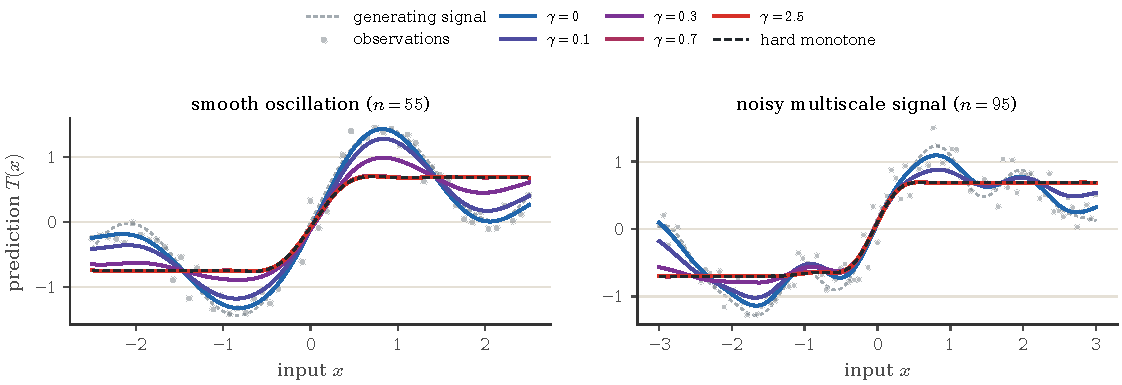
\includegraphics[width=\linewidth]{figures/monge-gap-kernel-regression/paths.pdf}
	\caption{\emph{A quadratic Monge-gap penalty traces a convex kernel-regression path toward monotonicity.} Gray dots are the observations and the light dashed curve is the generating signal. Colored curves solve~\eqref{eq-monge-gap-kernel-ridge} for increasing $\gamma$, from ordinary kernel ridge regression in blue to an almost monotone fit in red; the black dashed curve solves the corresponding hard monotonicity-constrained problem. The second experiment uses more points, stronger noise and a more oscillatory signal.}
	\label{fig:monge-gap-kernel-regression}
\end{figure}


%%%%%%%%%%%%%%%%%%%%%%%%%%%%%%%%%%%%%%%%%%%%%%%%%%%%%%%%%%%%%%%%%%%%%%%%%%%
\section{\texorpdfstring{$c$}{c}-Cyclical Monotonicity}
\index{cyclic!monotonicity}% strictindex
\label{sec-cyclical-monotonicity}

Cyclical monotonicity is the local geometric fingerprint of optimality. It converts a global minimization problem into finite exchange inequalities and is the bridge from Kantorovich plans to convex potentials.
\index{convex!potential}% strictindex

Optimal transport plans behave well when one looks at any finite sub-collection of points in their support: the restriction is still an optimal matching for those points alone. For finitely supported marginals this is immediate, and it leads to the notion of $c$-cyclical monotonicity.
\index{plan!transport}% strictindex
\index{c-cyclical monotonicity}% strictindex

\paragraph{Support and $c$-cyclical monotonicity.}
\index{cyclic!monotonicity}% strictindex

The support of a coupling is the topological support introduced in Definition~\ref{def:support}, now applied to a Radon measure on $\Xx\times\Yy$. Thus $(x,y)\in\supp(\pi)$ exactly when every open neighborhood of $(x,y)$ has positive $\pi$-mass.
\index{Radon measure}% strictindex

\begin{defn}[$c$-cyclical monotonicity]\label{def:ccm}
\index{cyclic!monotonicity}% strictindex
\index{c-cyclical monotonicity}% strictindex
	A set $\Gamma\subset\Xx\times\Yy$ is $c$-cyclically monotone if, for every $k\geq2$, every finite family $(x_i,y_i)_{i=1}^k\subset\Gamma$ and every permutation $\sigma$ of $\{1,\ldots,k\}$,
	\[
		\sum_{i=1}^k c(x_i,y_i)
		\leq
		\sum_{i=1}^k c(x_i,y_{\sigma(i)}).
	\]
\end{defn}

Any permutation is a product of cycles, so it suffices to verify the inequality for cyclic permutations,
\[
	\sum_{i=1}^k c(x_i,y_i)
	\leq
	\sum_{i=1}^k c(x_i,y_{i+1}),
	\qquad y_{k+1}=y_1.
\]

\paragraph{Optimal matching to optimal transport.}
\index{matching!optimal}% strictindex

Let the marginals be uniform on $n$ points, $\al=\frac1n\sum_{i=1}^n\delta_{x_i}$ and $\be=\frac1n\sum_{i=1}^n\delta_{y_i}$. By Corollary~\ref{cor-kantorovich-matching}, there exists an optimal plan induced by a permutation. Its support $\Gamma=\{(x_i,y_{\sigma(i)})\}_i$ is $c$-cyclically monotone: otherwise exchanging the finitely many targets along a violating cycle would lower the matching cost. The following theorem, in the spirit of Rockafellar's cyclic-monotonicity theorem~\cite{rockafellar2015convex}, says that the same finite-exchange condition holds for any optimal coupling, not only for finite uniform matchings.
\index{optimal coupling}% strictindex
\index{optimal plan}% strictindex
\index{cyclic!monotonicity}% strictindex
\index{matching!uniform}% strictindex

\begin{thm}[Optimal plans are $c$-cyclically monotone]\label{thm:opt_ccm}
		Assume that $c:\Xx\times\Yy\to[0,+\infty)$ is continuous and that the Kantorovich value is finite. For any optimal plan $\pi$ solving~\eqref{eq-mk-generic}, $\supp(\pi)$ is $c$-cyclically monotone.
\index{Kantorovich!problem}% strictindex
\end{thm}
\begin{proof}
	We prove the contrapositive. Suppose that $\supp(\pi)$ is not $c$-cyclically monotone. Then there exist points $(x_i,y_i)_{i=1}^k$ in the support and a permutation $\sigma$ such that $\sum_i c(x_i,y_i)>\sum_i c(x_i,y_{\sigma(i)})$.
	By continuity of $c$, after shrinking neighborhoods $U_i\ni x_i$ and $V_i\ni y_i$, the same strict inequality holds uniformly for every choice of points in these neighborhoods:
	\[
		\sum_i c(u_i,v_i)
		>
		\sum_i c(u_i,\tilde v_{\sigma(i)})
		\qquad
		(u_i\in U_i,\ v_i\in V_i,\ \tilde v_{\sigma(i)}\in V_{\sigma(i)}).
	\]
		Choose the sets so that $m_i\eqdef\pi(U_i\times V_i)>0$. Taking
		\(0<\lambda\leq\left(\sum_{i=1}^k\frac1{m_i}\right)^{-1}\)
		ensures that the scaled restrictions
		\(\pi_i=\lambda\frac{\pi|_{U_i\times V_i}}{m_i}\)
		have common mass $\lambda$ and satisfy $\sum_i\pi_i\leq\pi$, even if some rectangles overlap. Let $\al_i=(P_\Xx)_\sharp\pi_i$ and $\be_i=(P_\Yy)_\sharp\pi_i$, and define $\tilde\pi=\pi-\sum_i\pi_i+\sum_i(\al_i\otimes\be_{\sigma(i)})/\lambda$.
	The removed and reinserted first marginals are both $\sum_i\al_i$, and the removed and reinserted second marginals are both $\sum_i\be_i$ because $\sigma$ is a permutation. Hence $\tilde\pi\in\Couplings(\al,\be)$. Integrating the uniform strict inequality against the product probability $\otimes_i(\pi_i/\lambda)$ shows that the reinserted crossed terms have strictly smaller cost than the removed diagonal terms. This contradicts the optimality of $\pi$.
\end{proof}

\paragraph{Monotonicity.}

Assume the optimal plan is induced by a measurable map $T:\Xx\to\Yy$, meaning that $\pi=(\Id,T)_\sharp\al$. There is a set $G\subset\Xx$ of full $\al$-measure such that $(x,T(x))\in\supp(\pi)$ for every $x\in G$. For any $x_1,\ldots,x_k\in G$, cyclical monotonicity reads
\index{optimal plan}% strictindex
\index{cyclic!monotonicity}% strictindex
\[
	\sum_{i=1}^k c(x_i,T(x_i))
	\leq
	\sum_{i=1}^k c(x_i,T(x_{i+1})),
	\qquad x_{k+1}=x_1.
\]
For $c(x,y)=\frac12\norm{x-y}^2$, taking $k=2$ gives $\dotp{T(x)-T(y)}{x-y}\geq0$ for every $x,y\in G$, so the optimal representative of $T$ is monotone on $G$. Brenier's theorem adds that, when $\al$ is absolutely continuous, $T=\nabla\phi$ almost everywhere for a convex potential $\phi$. The converse fails in dimension $d\geq2$: as shown by the rotation example in the Monge section, a small rotation is monotone yet not a gradient.
\index{Brenier!theorem}% strictindex
\index{convex!potential}% strictindex

\paragraph{One dimension.}
\index{one-dimensional!transport}% strictindex
\index{monotone!rearrangement}% strictindex

In one space dimension, with cost $c(x,y)=|x-y|^p$, the two-point inequality becomes
\[
	|x-T(x)|^p+|y-T(y)|^p
	\leq
	|x-T(y)|^p+|y-T(x)|^p,
\]
For $p>1$, strict convexity implies that a reversed pair $x<y$ and $T(x)>T(y)$ violates this inequality. Hence every optimal map is nondecreasing on the full-measure transport set, recovering the classical monotone rearrangement. For $p=1$, uncrossing is non-strict: the monotone rearrangement remains optimal, but other optimal maps and non-deterministic plans can occur, as in the book-shifting example of Remark~\ref{rem-kantorovich-book-shifting}.
\index{monotone!rearrangement}% strictindex

The coupling formalism now provides a well-posed convex relaxation together with structural certificates for its optimizers. The next chapter specializes the cost to powers of a metric and turns these optimal values into a geometry on probability measures.

%%%%%%%%%%%%%%%%%%%%%%%%%%%%%%%%%%%%%%%%%%%%%%%%%%%%%%%%%%%%%%%%%%%%%%%%%%%
